\documentclass[11pt]{amsart}
\usepackage[T1]{fontenc}
\usepackage{lmodern,amsmath,amssymb,amsthm,mathtools,microtype,booktabs,array,longtable}
\usepackage[margin=1.06in]{geometry}
\usepackage{tikz}
\usepackage[hidelinks]{hyperref}
\hypersetup{pdftitle={Finite-Use Geometry and Learning of Ordered Binary Quantum Measurements},pdfauthor={Qian Qi}}
\emergencystretch=2em
\numberwithin{equation}{section}
\newtheorem{theorem}{Theorem}[section]
\newtheorem{lemma}[theorem]{Lemma}
\newtheorem{proposition}[theorem]{Proposition}
\newtheorem{corollary}[theorem]{Corollary}
\theoremstyle{definition}\newtheorem{definition}[theorem]{Definition}
\theoremstyle{remark}\newtheorem{remark}[theorem]{Remark}
\newcommand{\Q}{\mathbb Q}\newcommand{\R}{\mathbb R}\newcommand{\C}{\mathbb C}\newcommand{\N}{\mathbb N}\newcommand{\Z}{\mathbb Z}\newcommand{\E}{\mathbb E}
\newcommand{\ip}[2]{\langle #1,#2\rangle}\newcommand{\norm}[1]{\lVert #1\rVert}
\newcommand{\epsc}{\varepsilon_{\mathrm c}}
\DeclareMathOperator{\osc}{osc}\DeclareMathOperator{\spanop}{span}\DeclareMathOperator{\End}{End}\DeclareMathOperator{\diag}{diag}\DeclareMathOperator{\tr}{tr}\DeclareMathOperator{\rad}{rad}\DeclareMathOperator{\TV}{TV}
\title[Finite-use measurement geometry and learning]{Finite-Use Geometry and Learning of Ordered Binary Quantum Measurements}
\author{Qian Qi}
\date{4 October 2026}
\subjclass[2020]{Primary 81P15, 81P47; Secondary 94A17, 81P70}
\begin{document}
\raggedbottom
\begin{abstract}
We study the full body of ordered binary quantum measurements with
classical output and no residual quantum output. A regularized
Sylvester form at the midpoint of two effects is comparable, with
explicit dimension-dependent constants, to their finite-use adaptive
distance, including arbitrary references and every spectral rank.
In each fixed input dimension $d$, the small-error covering number
has order
\mbox{$N^{d^2/2}[\log(N+2)]^{\lfloor d/2\rfloor}\delta^{-d^2}$}.
Uniform volume bounds for actual operational balls and a nested
endpoint integral account for the logarithmic multiplicity.
We construct a common learner on the entire matrix body with
$Cd^4N\delta^{-2}\log(d/\eta)$ training calls for error $\delta$ in
the future-$N$ adaptive distance and failure probability at most $\eta$.
This learning guarantee holds for all $d,N\ge1$, sufficiently small absolute
$\delta>0$, and $0<\eta\le1/8$; each entangled block has at most $N$
calls. A scalar converse makes the dependence on horizon, error, and
confidence optimal for every fixed $d$. Simultaneous endpoint
calibration controls the variance introduced by two-dimensional
compressions, where a noise-adapted qubit learner applies.
A deterministic finite rational construction attains the covering
order, with exhaustive computation accounted for separately from
the reusable payload. All boundary cases are included.
\end{abstract}
\maketitle
\section{Introduction}

Repeated observations impose different resolutions on different
perturbations of a quantum measurement. An interior change of an
eigenvalue is resolved on the scale $N^{-1/2}$, whereas a rotation of
a projective measurement can be resolved on the scale $N^{-1}$.
The two scales meet at singular effects and repeated eigenvalues.
We determine the resulting geometry on a compact matrix body, calculate
its description entropy, and construct a common learning procedure
whose loss is the distinguishability of all future experiments with
at most $N$ uses.

Fix a finite input dimension $d$ and consider
\[
 \mathfrak E_d=\{E=E^*\in M_d(\C):0\preceq E\preceq I_d\}.
\]
The effect $E$ specifies the memoryless ordered binary measurement
\[
 \mathcal M_E(\rho)=\operatorname{tr}(E\rho)|1\rangle\langle1|
       +\operatorname{tr}((I_d-E)\rho)|0\rangle\langle0|.
\]
The input is consumed and the output is classical. The distance $d_N$
is the supremum of the unhalved trace norm between the final states
of a common experiment with at most $N$ calls. The experiment may
entangle its inputs, retain an arbitrary reference and quantum memory,
use feedback, and stop publicly. Thus $0\le d_N\le2$; classical total
variation is one half of the corresponding classical trace norm.
The nonadaptive restriction $d_N^{\rm na}$ retains entangled input
blocks and references and omits feedback between calls.

\subsection{An intrinsic comparison and its entropy}
For $E,F\in\mathfrak E_d$ put
\[
 M=\tfrac12(E+F),\qquad H=F-E,\qquad V=M(I_d-M),
\]
and define the midpoint modulus
\[
 Q_N(E,F)^2=N\langle H,
       (L_V+R_V+N^{-1}\operatorname{Id})^{-1}H\rangle_{\rm HS}.
\]
The inverse acts on the real Hilbert space of Hermitian matrices.
Theorem~\ref{thm:matrixmetric76} proves, for every $d,N\ge1$,
\begin{equation}\label{eq:intrometric77}
 \frac{\min\{1,Q_N(E,F)\}}{8192d}
 \le d_N^{\rm na}(\mathcal M_E,\mathcal M_F)
 \le d_N(\mathcal M_E,\mathcal M_F)
 \le\min\{2,8Q_N(E,F)\}.
\end{equation}
No spectral margin or multiplicity assumption is imposed. In particular
$d_N\le65536d\,d_N^{\rm na}$. This is a fixed-dimensional comparison
of optimal values. The modulus $Q_N$ is neither identified with an
optimal value nor assumed to satisfy a triangle inequality.

A horizontal measurement dilation yields the adaptive tangent bound.
A regularized Sylvester equation separates an arbitrary tangent from a
remainder controlled by the hybrid inequality. Operator concavity of
$G(I_d-G)$ then integrates the tangent bound along a finite segment,
including boundary endpoints. The converse uses Bernoulli inputs and
exact two-dimensional compressions. All required qubit statements and
their proofs are included below.

Let $\mathcal C_N(\mathfrak E_d,\delta)$ denote the least number of
legal memoryless binary centres needed to cover the body in $d_N$.
For every fixed $d$, Theorem~\ref{thm:matrixcover76} gives
\begin{equation}\label{eq:introentropy77}
 \mathcal C_N(\mathfrak E_d,\delta)
 \asymp_d N^{d^2/2}[\log(N+2)]^{\lfloor d/2\rfloor}\delta^{-d^2},
 \qquad N\ge1,\quad0<\delta\le\delta_d.
\end{equation}
The positive cap $\delta_d$ and the comparison constants may depend
on $d$. The proof first bounds the weighted volume of actual
operational balls uniformly over every boundary stratum. The total
volume is then a spectral integral whose ordered endpoint sectors have
cumulative exponents $S_j^2/2$, where $S_j$ is a signed prefix sum.
Balanced prefixes and matching nested endpoint boxes produce the
logarithmic multiplicity $\lfloor d/2\rfloor$.

\subsection{Learning with a future operational loss}
The statistical problem supplies calls to an unknown effect, without
its matrix entries. For every fixed $d$, Theorem~\ref{thm:matrixlearning77}
constructs one learner, common to all $E\in\mathfrak E_d$, satisfying
\begin{equation}\label{eq:introlearning77}
 \sup_E\mathbb P_E\{d_N(\mathcal M_E,\mathcal M_{\widehat E})
                         >\delta\}\le\eta,
 \qquad
 M\le C_d N\delta^{-2}\log(1/\eta).
\end{equation}
Here $N\ge1$, $0<\delta\le\delta_0$ for an absolute $\delta_0>0$,
and $0<\eta\le1/8$.
The bound on the training calls $M$ holds on every record. Each
entangled block uses at most $N$ calls. A scalar Bernoulli subfamily
gives the matching lower order even for arbitrary reference-assisted
adaptive training. More precisely, the upper bound is
$Cd^4N\delta^{-2}\log(d/\eta)$ with an absolute $C$.
The dependence on $d$ is not asserted to be optimal.

The construction begins with a qubit learner for unknown bias,
contrast, and direction. Independent fair signs remove the bias from
GHZ parity observations. A dyadic amplitude search stops at its first
rejected scale, preserving a small-cone invariant; fresh observations
complete the direction and endpoint estimates. Its confidence ledger
controls both exceptional records and the maximum training cost.

For a general matrix effect, an additional calibration stage is
essential. It estimates the two support boundaries in relative
Loewner order at scale $N^{-1}$ and controls the absolute matrix error
at scale $N^{-1/2}$. In the calibrated eigenbasis, these two guarantees
control the extra variance introduced by every two-dimensional
compression. Qubit learning on those compressions then gives
compatible matrix coordinates in the regularized quadratic form.
Projection onto the legal effect body completes the estimate. The
calibration and compression budgets are summed conditionally on the
observed record, with no additional $\log N$ factor.

\subsection{Deterministic descriptions and resources}
Theorem~\ref{thm:matrixcodec77} gives a deterministic finite rational
codebook at the order in \eqref{eq:introentropy77}. Its greedy rule
uses exact comparisons of $Q_N^2$ on a finite legal matrix grid.
The operational separation in \eqref{eq:intrometric77} controls its
cardinality, and an inward rounding map gives coverage at every rank.
The encoder and decoder reproduce the same dictionary from the public
parameters, with no supplied custom dictionary. Every fixed-length
word decodes to a legal effect. The required payload is
\[
 \frac{d^2}{2}\log_2N+
 \lfloor d/2\rfloor\log_2\log(N+2)
             +d^2\log_2(1/\delta)+O_d(1).
\]
The construction is finite and exact; its enumeration cost is large.
Optimal payload length does not imply efficient classical computation.
The direct qubit code remains available with its own detailed resource
accounting. Corollary~\ref{cor:matrixlearnedcode77} combines the common
learner with this exact encoder, attaining the learning and payload
orders simultaneously without additional calls to the unknown device.

\subsection{Prior work and organization}
Horizontal Kraus gauges, channel-extension metrology, and integration
of local distinguishability have established antecedents
\cite{FI76,DKG67,DM76,KGAD76,YF76,SD76}.
Inverse-Sylvester geometry and spectral matrix integration are likewise
classical \cite{Dittmann76,SZGeom76}. The explicit closed-body
midpoint comparison, its nested endpoint entropy, and learning under
the future operational loss are the theorem objects studied here.

Mele--Bittel \cite{MB67} and
Zambrano--Ramos-Calderer--Kueng \cite{ZRK76} already provide common
estimators for unknown measurements in one-use losses. Their access,
rank, dimension, and confidence statements are compared at theorem
level in Section~\ref{sec:matrixcomparison76}. The distinction in
\eqref{eq:introlearning77} is the dependence on the future horizon
under the anisotropic loss $d_N$. The phase-estimation components
have antecedents in \cite{HB76,KLY76}; the conditional construction
used here is proved directly.

The matrix comparison and entropy are followed by the qubit learning
construction, its extension to fixed matrix dimension, and the exact
codebook theorem. The later qubit geometry and the final prerequisite
appendix make the focused article self-contained. The complete
research edition preserves the earlier instrument, preparation,
coherent, readout, stochastic-realization, arithmetic, and causal
developments with their original hypotheses and proofs. The
structural companion treats repeatable nondisturbing classical
observations and retains that separate physical interface.

\section{Matrix geometry in arbitrary input dimension}
\label{sec:matrixmetric76}

The binary effect body has a finite-use description that does not
require eigenvector coordinates.  Its regularization is the same at
every spectral rank, and two-dimensional compressions supply lower
witnesses for the full matrix problem.  Throughout this section
$d,N\ge1$ are integers and
\begin{equation}\label{eq:matrixbody76}
 \mathfrak E_d=\{E\in\End(\C^d):E=E^*,\ 0\preceq E\preceq I_d\}.
\end{equation}
The measurement $\mathcal M_E$ has the ordered effects $E,I_d-E$
and no residual quantum output.  The distance $d_N$ has the same
reference-assisted adaptive meaning as in
Theorem~\ref{thm:biasedmetric75}.  Write $d_N^{\rm na}$ for its
restriction to nonadaptive experiments, allowing entanglement across
the calls and a retained reference.  These experiments may depend on
the known pair of hypotheses.

Put $\tau=N^{-1}$ and $V_E=E(I_d-E)$.  On the real Hilbert space
of Hermitian matrices with Hilbert--Schmidt inner product, define
\begin{align}
 \mathcal A_E(H)&=V_EH+HV_E+\tau H,
                                      \label{eq:matrixoperator76}\\
 g_{N,E}(H)^2&=N\ip{H}{\mathcal A_E^{-1}(H)}_{\rm HS}.
                                      \label{eq:matrixform76}
\end{align}
The operator $\mathcal A_E$ is strictly positive, including at a
singular effect.  For a pair $E,F$ set
\begin{equation}\label{eq:matrixmodulus76}
 M=\tfrac12(E+F),\qquad H=F-E,\qquad
 Q_N(E,F)=g_{N,M}(H).
\end{equation}
In any orthonormal eigenbasis of $M$, with eigenvalues $m_i$ and
$v_i=m_i(1-m_i)$, this is
\begin{equation}\label{eq:matrixcoordinates76}
 Q_N(E,F)^2=N\sum_{i,j=1}^d
                \frac{|H_{ij}|^2}{v_i+v_j+N^{-1}}.
\end{equation}
Definition~\eqref{eq:matrixmodulus76} makes the expression independent
of all choices at repeated eigenvalues.  We use it as a comparison
modulus; a triangle inequality for $Q_N$ is not required.

The inverse Sylvester operator is familiar from the Bures metric
$g^{\rm B}$ on the positive definite cone \cite{Dittmann76}.
Its normalization gives the algebraic identity
\[
 g_{N,E}(H)^2=2N\,g^{\rm B}_{V_E+\tau I_d/2}(H,H).
\]
Here $H$ remains the effect tangent; the differential of the
variance map $E\mapsto V_E$ is $H-EH-HE$.

\begin{theorem}[Finite-use geometry of the matrix effect body]
\label{thm:matrixmetric76}
For every $E,F\in\mathfrak E_d$,
\begin{equation}\label{eq:matrixmetric76}
 \frac1{8192d}\min\{1,Q_N(E,F)\}
 \le d_N^{\rm na}(\mathcal M_E,\mathcal M_F)
 \le d_N(\mathcal M_E,\mathcal M_F)
 \le\min\{2,8Q_N(E,F)\}.
\end{equation}
The constants are uniform in the horizon and in both effects,
without a spectral margin or a condition on eigenvalue multiplicities.
The adaptive upper bound permits arbitrary retained references,
common feedback, and bounded public stopping.  Each lower witness
uses inputs in one fixed subspace of dimension at most two.  Moreover,
\begin{equation}\label{eq:matrixoneuse76}
 d_1(\mathcal M_E,\mathcal M_F)=2\|E-F\|_{\rm op}.
\end{equation}
\end{theorem}

The theorem includes every rank of projection and all of the
intermediate singular strata.  The variance $E(I_d-E)$, rather than
the smallest eigenvalue of either outcome, determines the matrix
weights.  The factor $N^{-1}$ makes the formula finite on the entire
closed body.  The proof first establishes a path inequality valid for
every common adaptive tester, and then obtains the converse from
one- and two-dimensional experiments.

\subsection{A horizontal measurement dilation}

Kraus-gauge bounds for channel estimation were developed in
\cite{FI76,DKG67,DM76}.  Their integration along channel paths
appears in \cite[Section~III, equation~(26)]{YF76} and, with
general adaptive bounds, in \cite[Section~IV.A]{SD76}.  We use an
explicit horizontal lift for binary effects and control the
finite-horizon regularization by a trace-norm remainder.

\begin{lemma}[Horizontal derivative and regularized path bound]
\label{lem:matrixpath76}
Every continuously differentiable path $G:[0,1]\to\mathfrak E_d$
satisfies
\begin{equation}\label{eq:matrixpath76}
 d_N(\mathcal M_{G(0)},\mathcal M_{G(1)})
       \le4\int_0^1 g_{N,G(t)}(G'(t))\,dt.
\end{equation}
\end{lemma}
\begin{proof}
We begin with an interior effect $G$, so that $G$ and $I_d-G$
are invertible.  Set $S=\sqrt{G(I_d-G)}$.  For a Hermitian matrix
$K$ put $H_0=SK+KS$.  At the two factors
$A_1=\sqrt G$, $A_0=\sqrt{I_d-G}$ prescribe derivatives
\begin{equation}\label{eq:horizontalderivatives76}
 B_1=\sqrt{I_d-G}\,K,\qquad B_0=-\sqrt G\,K.
\end{equation}
They obey
\begin{align}
 A_1^*B_1+B_1^*A_1&=H_0,&
 A_0^*B_0+B_0^*A_0&=-H_0,\notag\\
 \sum_{y=0}^1 A_y^*B_y&=0,&
 \sum_{y=0}^1 B_y^*B_y&=K^2.
                                      \label{eq:horizontalidentities76}
\end{align}

These tangent equations can be realized by genuine dilations.
Let $G_1(s)=G+sH_0$, $G_0(s)=I_d-G-sH_0$ for $s$ in a
sufficiently small open interval, and put $R_y(s)=\sqrt{G_y(s)}$.
The first line of \eqref{eq:horizontalidentities76} implies that
\[
 T_y=(B_y-R_y'(0))R_y(0)^{-1}
\]
is anti-Hermitian.  Indeed, multiplying $T_y+T_y^*$ on the left
and right by $R_y(0)$ gives, with $R=R_y(0)$,
\[
 R(T_y+T_y^*)R=RB_y+B_y^*R-(RR_y'(0)+R_y'(0)R)=0,
\]
by differentiating $R_y(s)^2=G_y(s)$.  Thus
$\widetilde A_y(s)=\exp(sT_y)R_y(s)$ has derivative $B_y$ at
zero and satisfies
$\widetilde A_y(s)^*\widetilde A_y(s)=G_y(s)$ exactly.  A measurement
isometry is
\[
 W(s)\psi=\sum_{y=0}^1
              |y\rangle_C|y\rangle_L\widetilde A_y(s)\psi.
\]
Here $C$ is the observed outcome, and $L$ and the factor space of
$\widetilde A_y$ are environments.  Tracing the environments
implements $\mathcal M_{G(s)}$, also on inputs entangled with a
reference.  At zero, \eqref{eq:horizontalidentities76} gives
\begin{equation}\label{eq:horizontaloverlap76}
 W^*\dot W=0,\qquad \dot W^*\dot W=K^2.
\end{equation}

The horizontal Kraus condition has the antecedents
\cite[Theorems~4--5]{FI76}. Its adaptive channel-extension form is
$F_N\le4N\|\alpha\|$ when $\beta=0$; see
\cite[equation~(9)]{DM76} and \cite[equations~(5)--(10)]{KGAD76}.
In the present lift $\alpha=K^2$ and $\beta=0$. We give the cancellation
explicitly for this binary measurement.

Fix a common tester with $N$ slots.  Purify its initial state and
all intervening operations, and retain the measurement environments
only for this comparison; neither the outcome copy nor the factor
environment is accessible to the tester.  The derivative of its final purification
in the direction $H_0$ is the sum of $N$ terms, each having one
differentiated occurrence of $W$.  The terms are mutually orthogonal.
For two different differentiated slots, cancel the common isometries
after the later slot; the remaining overlap contains
$W^*\dot W\otimes I=0$.  Each term has norm at most
$\|\dot W\|_{\rm op}=\|K\|_{\rm op}$, independently of the
reference and memory dimensions.  Hence the derivative of the
purification has norm at most $\sqrt N\|K\|_{\rm op}$.
The pure-state trace-norm derivative bound, followed by contraction
under the partial trace, bounds the observed output derivative by
\begin{equation}\label{eq:horizontaltangent76}
 2\sqrt N\|K\|_{\rm op}.
\end{equation}
A publicly stopped tester is padded to $N$ slots by calls on fixed
dummy inputs, whose outcomes and environments are both discarded.  The same purification
argument then applies to its original output.  Classical feedback is
included by purifying the common controlled operations.

Now let $H$ be an arbitrary Hermitian tangent at $G$, and set
$\kappa=N^{-1/2}$.  There is a unique Hermitian solution of
\begin{equation}\label{eq:regularizedsylvester76}
 SK+KS+\kappa K=H.
\end{equation}
Write $H=H_0+R$, with $H_0=SK+KS$ and $R=\kappa K$.
Both are legitimate tangents at the interior effect $G$.  The
derivative of a fixed tester's output is linear in the inserted
channel tangent.  The part arising from $H_0$ is bounded by
\eqref{eq:horizontaltangent76}.  The part arising from $R$ is
bounded by $2N\|R\|_{\rm op}$.  To verify the latter bound,
the one-call tangent has two opposite reference blocks
\[
 B_\rho=\tr_A[(R\otimes I)\rho],\qquad -B_\rho.
\]
Duality against Hermitian contractions gives
$\|B_\rho\|_1\le\|R\|_{\rm op}$ for every input state.
Insert this tangent into each of the $N$ slots in turn; all
subsequent common channels contract the Hermitian trace norm.
This proves the bound for its sum.  Thus the actual tangent $H$
has output derivative bounded by
\begin{equation}\label{eq:regularizedtangent76}
 2\sqrt N\|K\|_{\rm op}+2N\|R\|_{\rm op}
                         =4\sqrt N\|K\|_{\rm op}.
\end{equation}
The splitting is used only for the differential at an interior
effect; it does not postulate a physical mixture realizing the
entire path.

In an eigenbasis of $G$, with $v_i=g_i(1-g_i)$, equation
\eqref{eq:regularizedsylvester76} reads
\[
 K_{ij}=\frac{H_{ij}}{\sqrt{v_i}+\sqrt{v_j}+\kappa}.
\]
Since $(\sqrt{v_i}+\sqrt{v_j}+\kappa)^2\ge v_i+v_j+\tau$,
\begin{equation}\label{eq:regularizedformbound76}
 \sqrt N\|K\|_{\rm op}
 \le\sqrt N\|K\|_{\rm HS}
 \le g_{N,G}(H).
\end{equation}
The integration of local distinguishability has direct antecedents:
\cite[Section~III, equation~(26), PDF version~3]{YF76} treats the
parallel path bound, and
\cite[Section~IV.A, equations~(14)--(22)]{SD76} applies adaptive
metrological estimates. Here the regularized binary Sylvester split
and its residual produce the explicit integrand.
For an interior path, integrate the resulting output derivative
bound for each fixed tester, and then take the supremum.  This
proves \eqref{eq:matrixpath76} without exchanging a supremum
with a derivative.

For a path in the closed body, apply the result to
$G_\epsilon(t)=(1-2\epsilon)G(t)+\epsilon I_d$, where
$0<\epsilon<1/2$.  At fixed $N$, the form
$g_{N,G}(H)$ is continuous on the whole body and bounded above
by $N\|H\|_{\rm HS}$.  The integrals therefore converge as
$\epsilon\downarrow0$.  The hybrid inequality
$d_N(\mathcal M_E,\mathcal M_F)\le2N\|E-F\|_{\rm op}$
gives continuity of the distances at both endpoints.  Passing to
the limit proves the asserted closed-body statement.
\end{proof}

\subsection{The midpoint comparison}

\begin{proof}[Proof of Theorem~\ref{thm:matrixmetric76}]
For the upper bound use $G(t)=(1-t)E+tF$.  The map
$G\mapsto V_G=G-G^2$ is operator concave.  For $0<t\le1/2$,
write $G(t)=(1-2t)E+2tM$ and discard the positive multiple of
$V_E$ in the concavity inequality.  Applying the same argument
from the other endpoint gives
\begin{equation}\label{eq:midpointvariance76}
 V_{G(t)}\succeq a(t)V_M,\qquad
             a(t)=2\min\{t,1-t\}.
\end{equation}
For a positive matrix $D$ and a Hermitian matrix $X$,
\[
 \langle X,(L_D+R_D)X\rangle_{\rm HS}
       =2\operatorname{tr}(DX^2)\ge0.
\]
Thus left-plus-right multiplication preserves the stated order on the
real Hilbert space of Hermitian matrices.  Since $a(t)\le1$,
$\mathcal A_{G(t)}\succeq a(t)\mathcal A_M$.
Inverting positive operators reverses their order, whence
\[
 g_{N,G(t)}(H)\le a(t)^{-1/2}Q_N(E,F).
\]
The scalar factor has integral $2$ on $[0,1]$.
Lemma~\ref{lem:matrixpath76} yields $d_N\le8Q_N$;
the trace-norm bound $d_N\le2$ gives the stated upper estimate.

For the lower bound choose any orthonormal eigenbasis $e_i$ of
$M$ and put
\begin{equation}\label{eq:matrixentries76}
 q_{ij}=|H_{ij}|\sqrt{\frac N{v_i+v_j+\tau}},
                 \qquad Q_N^2=\sum_{i,j}q_{ij}^2.
\end{equation}
Repeated input $e_i$ gives Bernoulli probabilities
$s=m_i-H_{ii}/2$, $t=m_i+H_{ii}/2$.  Their variances satisfy
\[
 \max\{s(1-s),t(1-t)\}
 \le s(1-s)+t(1-t)\le2m_i(1-m_i).
\]
Lemma~\ref{lem:bernoulliproduct75} therefore gives
\begin{equation}\label{eq:matrixdiagonallower76}
 d_N^{\rm na}(\mathcal M_E,\mathcal M_F)
                            \ge\tfrac1{64}\min\{1,q_{ii}\}.
\end{equation}

For $i\ne j$, restrict each input to
$\mathcal S=\spanop\{e_i,e_j\}$.  The resulting channels have
the compressed effects $E_{\mathcal S},F_{\mathcal S}$, including
on inputs entangled with a retained reference.  Their midpoint is
$M_{\mathcal S}=\diag(m_i,m_j)$.  Write their spectral data as
$(p,q,u)$ and $(p',q',v)$ in the notation of
Section~\ref{sec:biasedmetric75}, with gaps $r,r'$ and angle $h$
when both gaps are positive.  Put
\[
 V_E^{\mathcal S}=p(1-p)+q(1-q),\qquad
 V_F^{\mathcal S}=p'(1-p')+q'(1-q').
\]
For the compressed matrices the exact identity
\[
 V_{M_{\mathcal S}}=\tfrac12V_{E_{\mathcal S}}
              +\tfrac12V_{F_{\mathcal S}}
              +\tfrac14(F_{\mathcal S}-E_{\mathcal S})^2
\]
shows, on taking traces, that
\begin{equation}\label{eq:compressionvariance76}
 v_i+v_j+\tau\ge\tfrac12(V_E^{\mathcal S}+\tau),
 \qquad
 v_i+v_j+\tau\ge\tfrac12(V_F^{\mathcal S}+\tau).
\end{equation}
The scalar part of $F_{\mathcal S}-E_{\mathcal S}$ has zero
off-diagonal entry.  Its traceless part has operator norm
$|ru-r'v|/2$.  Decomposing this vector along the smaller radius
gives
\begin{align}
 |H_{ij}|&\le\tfrac12|r-r'|+\min\{r,r'\}\sin(h/2)\notag\\
 &\le\tfrac12\bigl(|p-p'|+|q-q'|+\min\{r,r'\}h\bigr).
                                      \label{eq:compressionoffdiagonal76}
\end{align}
When one radius is zero, the angular term is zero and the same
inequality holds without choosing its direction.  Each endpoint
variance is bounded by the appropriate $V_E^{\mathcal S}$ or
$V_F^{\mathcal S}$.  Equations
\eqref{eq:compressionvariance76}--\eqref{eq:compressionoffdiagonal76}
therefore imply
\begin{equation}\label{eq:compressionmodulus76}
 q_{ij}\le\frac1{\sqrt2}
 \left(T_N(p,p')+T_N(q,q')
       +\min\{K_N(p,q),K_N(p',q')\}h\right).
\end{equation}
The nonadaptive assertion of Theorem~\ref{thm:biasedmetric75}
applied to this compressed pair yields
\begin{equation}\label{eq:matrixoffdiagonallower76}
 d_N^{\rm na}(\mathcal M_E,\mathcal M_F)
                         \ge\tfrac1{8192}\min\{1,q_{ij}\}.
\end{equation}
Every such witness is a legitimate experiment for the original
effects by a fixed isometric embedding of $\mathcal S$.
Since $\max_{i,j}q_{ij}\ge Q_N/d$, taking the strongest of
\eqref{eq:matrixdiagonallower76} and
\eqref{eq:matrixoffdiagonallower76} proves the lower bound.
For $d=1$ only the diagonal argument is needed.

Finally, a one-use reference-assisted difference has output blocks
$B_\rho$ and $-B_\rho$, with
$B_\rho=\tr_A[((E-F)\otimes I)\rho]$.  Trace-norm duality
against Hermitian contractions gives
$\|B_\rho\|_1\le\|E-F\|_{\rm op}$.  An eigenstate of
$E-F$ at an extremal eigenvalue attains equality.  This proves
\eqref{eq:matrixoneuse76}.
\end{proof}

\begin{corollary}[Uniform comparison with nonadaptive experiments]
\label{cor:matrixadaptivity76}
For all $E,F\in\mathfrak E_d$ and all $N\ge1$,
\begin{equation}\label{eq:matrixadaptivity76}
 d_N(\mathcal M_E,\mathcal M_F)
           \le65536d\,d_N^{\rm na}(\mathcal M_E,\mathcal M_F).
\end{equation}
Here nonadaptive experiments may entangle all inputs and retain a
reference; they use no feedback between calls. The dimensional constant
comes from the maximum of $d^2$ weighted entries and is not optimized.
\end{corollary}
\begin{proof}
If $Q_N\le1$, divide the upper estimate $8Q_N$ by the lower
estimate $Q_N/(8192d)$.  If $Q_N\ge1$, the upper estimate is
$2$ and the lower estimate is $1/(8192d)$, which gives a smaller
constant.  The identical pair needs no division.
\end{proof}

\subsection{All spectral ranks and local forms}

\begin{lemma}[Spectral noncancellation in every rank]
\label{lem:matrixspectral76}
Let $\lambda_1(E)\ge\cdots\ge\lambda_d(E)$ and
$\lambda_1(F)\ge\cdots\ge\lambda_d(F)$ be the ordered spectra.
For every $1\le k\le d$,
\begin{equation}\label{eq:matrixspectrallower76}
 B_N(\lambda_k(E),\lambda_k(F))
                   \le d_N^{\rm na}(\mathcal M_E,\mathcal M_F).
\end{equation}
For effects diagonal in the same ordered orthonormal basis,
\begin{equation}\label{eq:matrixspectralupper76}
 d_N(\mathcal M_E,\mathcal M_F)
       \le\sum_{k=1}^d B_N(\lambda_k(E),\lambda_k(F)).
\end{equation}
\end{lemma}
\begin{proof}
Suppose $\lambda_k(E)\ge\lambda_k(F)$.  The span of the first
$k$ eigenvectors of $E$ intersects the orthogonal complement of
the first $k-1$ eigenvectors of $F$ in a nonzero subspace.  A unit
vector in that intersection has success probabilities
$s\ge\lambda_k(E)\ge\lambda_k(F)\ge t$ under the two
hypotheses.  The monotonicity in
Lemma~\ref{lem:bernoulliproduct75} implies
$B_N(s,t)\ge B_N(\lambda_k(E),\lambda_k(F))$.
Repeated use of this vector proves the first assertion; reverse
the hypotheses for the opposite ordering.  Multiplicities cause
no change in the dimension argument.

For the upper bound, first measure the common eigenbasis and then
produce a bit whose success probability is its corresponding
eigenvalue.  Supply $N$ independent bits in each of the $d$ rows
before the experiment.  Every common adaptive tester is a common
channel of these row arrays, including its reference blocks and
all publicly stopped histories.  The tensor-product triangle
inequality gives \eqref{eq:matrixspectralupper76}; unused row
bits are discarded.
\end{proof}

The following local comparison will permit volume estimates at
every boundary stratum.  It concerns matrices themselves and
does not require a coordinate chart for eigenvectors.

\begin{lemma}[Uniform local comparison of the variance forms]
\label{lem:matrixlocal76}
Set $W_G=G(I_d-G)+\tau I_d/2$.  For a Hermitian $H$, put
$q=g_{N,G}(H)$.  Then
\begin{equation}\label{eq:matrixrelative76}
 \|W_G^{-1/2}HW_G^{-1/2}\|_{\rm HS}\le2q.
\end{equation}
For either sign for which $G\pm H/2\in\mathfrak E_d$, one has
\begin{equation}\label{eq:matrixlocalperturbation76}
 \bigl\|W_G^{-1/2}(W_{G\pm H/2}-W_G)W_G^{-1/2}\bigr\|_{\rm op}
                       \le q+\tfrac34q^2.
\end{equation}
In particular, for $q\le1/4$,
\begin{equation}\label{eq:matrixlocalorder76}
 \tfrac12W_G\preceq W_{G\pm H/2}\preceq2W_G.
\end{equation}
Thus, if either $Q_N(E,F)\le1/4$ or
$g_{N,E}(F-E)\le1/4$, the midpoint and the fixed-endpoint
quadratic forms are comparable within factors $2$.
\end{lemma}
\begin{proof}
In an eigenbasis of $W_G$, with eigenvalues $w_i\ge\tau/2$,
\[
 \frac{w_i+w_j}{Nw_iw_j}\le4.
\]
Multiplying this inequality by
$N|H_{ij}|^2/(w_i+w_j)$ and summing proves
\eqref{eq:matrixrelative76}.  Put
$Z=W_G^{-1/2}HW_G^{-1/2}$.  The exact expansion
\[
 W_{G\pm H/2}-W_G
            =\pm\tfrac12(H-GH-HG)-\tfrac14H^2
\]
has normalized linear part
$\pm((I_d-2G)Z+Z(I_d-2G))/4$, since $G$ commutes with
$W_G$.  Its operator norm is at most $\|Z\|_{\rm op}/2\le q$.
The normalized quadratic part is $-ZW_GZ/4$.
Since $\tau\le1$, one has $\|W_G\|_{\rm op}\le3/4$, and
its norm is at most $3q^2/4$.  This proves
\eqref{eq:matrixlocalperturbation76} and hence
\eqref{eq:matrixlocalorder76}.  The same order holds for left
plus right multiplication, and inversion gives the quadratic-form
comparison.  Apply it first at $G=M$ or at $G=E$, respectively,
to obtain the final assertion.
\end{proof}

\section{Description entropy in arbitrary matrix dimension}
\label{sec:matrixentropy76}
The intrinsic comparison of Theorem~\ref{thm:matrixmetric76} permits
the full effect body to be treated without choosing eigenvector
coordinates near repeated spectra. Throughout this section the input
dimension $d\ge1$ is fixed. Constants may depend on $d$, but not on the
integer horizon $N\ge1$ or on the accuracy parameter.

Write $\mathcal C_N(\mathfrak E_d,\delta)$ for the covering number under
$d_N$, with centres in the same legal memoryless ordered binary
interface, and write $\mathcal C_N^{\mathrm{rat}}$ when the real and
imaginary parts of every matrix entry of each centre are rational.

\begin{theorem}[Entropy of the full effect body]\label{thm:matrixcover76}
For every integer $d\ge1$ there are constants $c_d,C_d,\delta_d>0$
such that, for all integers $N\ge1$ and all $0<\delta\le\delta_d$,
\begin{equation}\label{eq:matrixcover76}
\begin{split}
 c_d N^{d^2/2}[\log(N+2)]^{\lfloor d/2\rfloor}\delta^{-d^2}
 &\le \mathcal C_N(\mathfrak E_d,\delta)\\
 &\le \mathcal C_N^{\mathrm{rat}}(\mathfrak E_d,\delta)\\
 &\le C_d N^{d^2/2}[\log(N+2)]^{\lfloor d/2\rfloor}\delta^{-d^2}.
\end{split}
\end{equation}
Consequently the optimum fixed-length reusable description has length
\begin{equation}\label{eq:matrixbits76}
 \frac{d^2}{2}\log_2N
 +\lfloor d/2\rfloor\log_2\log(N+2)
 +d^2\log_2(1/\delta)+O_d(1).
\end{equation}
The estimates include all support and spectral multiplicities. The
rational-centre assertion here follows from a covering argument.
Theorem~\ref{thm:matrixcodec77} gives a deterministic finite exact
encoder and decoder attaining the same order in every dimension.
Theorem~\ref{thm:biasedcodec75} retains its separate direct construction
in dimension two. Computational cost is accounted for separately
from the number of transmitted bits.
\end{theorem}

For $d=1$, the result is the Bernoulli covering law
$N^{1/2}\delta^{-1}$. For $d=2$, it recovers
Theorem~\ref{thm:biasedcover75}. The next two cases have orders
$N^{9/2}\log(N+2)\delta^{-9}$ and
$N^8[\log(N+2)]^2\delta^{-16}$. The logarithmic power counts independent
nested approaches of paired eigenvalues to the two support endpoints.
We first establish a uniform measure estimate for actual operational
balls, and then evaluate the total measure.

\subsection{Operational balls and a regularized volume form}
Set $n=d^2$, $\tau=N^{-1}$ and
\[
 W_E=E(I-E)+\frac\tau2 I.
\]
As in Section~\ref{sec:matrixmetric76}, let
\begin{equation}\label{eq:matrixfixedform76}
 g_{N,E}(H)^2
 =N\langle H,(L_{W_E}+R_{W_E})^{-1}H\rangle_{\mathrm{HS}}
\end{equation}
on the real Hilbert space of Hermitian matrices. Let $G_{N,E}$ denote
this positive quadratic form in Hilbert--Schmidt orthonormal
coordinates, and define
\begin{equation}\label{eq:matrixmeasure76}
 \rho_N(E)=\sqrt{\det G_{N,E}},\qquad
 d\mu_N(E)=\rho_N(E)\,dE,
\end{equation}
The real orthonormal basis consists of $e_{ii}$ and, for $i<j$,
$(e_{ij}+e_{ji})/\sqrt2$ and $\mathrm i(e_{ij}-e_{ji})/\sqrt2$;
$dE$ is Lebesgue measure in these coordinates. The cutoff makes
$\rho_N$ positive and continuous on the whole closed body for each
$N$.

\begin{lemma}[Uniform volume of operational balls]\label{lem:matrixball76}
For fixed $d$ there are $a_d,A_d,r_d>0$ such that
\begin{equation}\label{eq:matrixball76}
 a_dr^{d^2}\le
 \mu_N\bigl(B_{d_N}(E,r)\bigr)
 \le A_dr^{d^2}
\end{equation}
for every $N\ge1$, every $E\in\mathfrak E_d$, and every
$0<r\le r_d$. Balls are taken inside $\mathfrak E_d$.
\end{lemma}
\begin{proof}
We make explicit the two local consequences of
Lemma~\ref{lem:matrixlocal76} that will be used. If $H$ is Hermitian and
$q=g_{N,E}(H)$, diagonalizing $W_E$ gives
\begin{equation}\label{eq:matrixnormalized76}
 \|W_E^{-1/2}HW_E^{-1/2}\|_{\mathrm{HS}}^2
 \le4q^2,
\end{equation}
since its eigenvalues $w_i$ are at least $\tau/2$ and
\[
 \frac{w_i+w_j}{Nw_iw_j}
                  =\tau(w_i^{-1}+w_j^{-1})\le4.
\]
For any legal $E+tH$, direct expansion yields
\[
 W_{E+tH}-W_E
 =\frac t2\bigl((I-2E)H+H(I-2E)\bigr)-t^2H^2.
\]
The matrices $E$ and $W_E$ commute, $\|I-2E\|_{\rm op}\le1$, and
$\|W_E\|_{\rm op}\le3/4$. Thus the norm of the normalized difference
is at most $2|t|q+3t^2q^2$. For $|t|\le1$ and $q$ below an absolute
constant, it follows that
\begin{equation}\label{eq:matrixvariancecomparison76}
 \tfrac12W_E\preceq W_{E+tH}\preceq2W_E.
\end{equation}
Loewner comparison passes to $L_W+R_W$ and, by inversion, to the
quadratic forms. It also gives
\begin{equation}\label{eq:matrixdensitycomparison76}
 2^{-n/2}\rho_N(E)\le\rho_N(E+tH)\le2^{n/2}\rho_N(E).
\end{equation}

Apply this comparison from an endpoint to the midpoint and from the
midpoint to either endpoint. Theorem~\ref{thm:matrixmetric76} then
provides constants $A,B,r_0>0$, depending only on $d$, such that
\begin{align}
 d_N(E,F)\le r&\ \Longrightarrow\
       g_{N,E}(F-E)\le Ar,\label{eq:matrixballupperellipse76}\\
 g_{N,E}(F-E)\le Br&\ \Longrightarrow\
       d_N(E,F)\le r,\label{eq:matrixballlowerellipse76}
\end{align}
for legal $E,F$ and $0<r\le r_0$. Decrease $r_0$ so that $Ar_0$
lies in the small-form range of \eqref{eq:matrixvariancecomparison76}.

Let $\omega_n$ be the Euclidean volume of the unit ball in $\R^n$.
The ellipsoid $g_{N,E}(H)\le u$ has Lebesgue volume
$\omega_nu^n/\rho_N(E)$. Equations
\eqref{eq:matrixballupperellipse76} and
\eqref{eq:matrixdensitycomparison76} therefore imply
\[
 \mu_N\bigl(B_{d_N}(E,r)\bigr)
                  \le2^{n/2}\omega_n(Ar)^n.
\]

For the lower bound we construct a full legal ellipsoid, including
when $E$ lies on a support boundary. Choose a small constant $a>0$
depending only on $d$, set $s=ar\tau$, and move towards the scalar
interior point:
\begin{equation}\label{eq:matrixinwardshift76}
 E_s=(1-2s)E+sI.
\end{equation}
Take $r_0$ sufficiently small that $s\le1/4$. Then
$sI\preceq E_s\preceq(1-s)I$. Since the displacement commutes with
$E$, its form is bounded by
\[
 g_{N,E}(E_s-E)^2
 =N\sum_i\frac{s^2(1-2\lambda_i)^2}
                    {2\lambda_i(1-\lambda_i)+\tau}
 \le d\frac{s^2}{\tau^2}=da^2r^2.
\]
Choose $a\sqrt d\le B/4$. By
\eqref{eq:matrixballlowerellipse76},
$d_N(E,E_s)\le r/4$.

Let $X=X^*$ satisfy $g_{N,E_s}(X)\le br$, with $b>0$ to be chosen.
Write $\ell_i$ for the eigenvalues of $E_s$ and
$w_i=\ell_i(1-\ell_i)+\tau/2$. Since $\ell_i\ge s$ and
$w_i\le\ell_i+\tau/2$, we have
\begin{align*}
 \|E_s^{-1/2}XE_s^{-1/2}\|_{\mathrm{HS}}^2
 &\le g_{N,E_s}(X)^2
       \max_{i,j}\frac{w_i+w_j}{N\ell_i\ell_j}\\
 &\le b^2r^2\left(\frac{2\tau}{s}
                         +\frac{\tau^2}{s^2}\right)
   =b^2\left(\frac{2r}{a}+\frac1{a^2}\right).
\end{align*}
The same bound holds with $I-E_s$ in place of $E_s$, because
$1-\ell_i\ge s$ and $w_i\le1-\ell_i+\tau/2$. Taking
$b\le a/4$ and $ar_0\le1$ makes both operator norms at most $1/2$.
Consequently every point of the entire ellipsoid
\[
 \mathcal A_s=\{E_s+X:g_{N,E_s}(X)\le br\}
\]
is a legal effect. Choose also $b\le B/4$. Equation
\eqref{eq:matrixballlowerellipse76} and the triangle inequality give
$\mathcal A_s\subset B_{d_N}(E,r)$. The density comparison about
$E_s$ and the exact ellipsoid volume now imply
\[
 \mu_N\bigl(B_{d_N}(E,r)\bigr)
           \ge2^{-n/2}\omega_n(br)^n.
\]
All choices depend only on $d$. This proves the assertion on every
boundary stratum as well as in the interior.
\end{proof}

\subsection{The total regularized volume}
\begin{proposition}[Nested endpoint accumulation]\label{prop:matrixvolume76}
For fixed $d\ge1$, uniformly over $N\ge1$,
\begin{equation}\label{eq:matrixvolume76}
 \mu_N(\mathfrak E_d)
       \asymp_d N^{d^2/2}[\log(N+2)]^{\lfloor d/2\rfloor}.
\end{equation}
\end{proposition}
\begin{proof}
In a spectral basis, the quadratic form has weight $N/(2w_i)$ on
the $i$th diagonal direction and weight $N/(w_i+w_j)$ on each of
the two Hilbert--Schmidt orthonormal real directions belonging to
$i<j$. Hence
\begin{equation}\label{eq:matrixdeterminant76}
 \rho_N(E)=2^{-d/2}N^{d^2/2}
       \prod_iw_i^{-1/2}\prod_{i<j}(w_i+w_j)^{-1}.
\end{equation}
We use the classical spectral change of variables
\cite{SZGeom76}. For a simple spectrum, differentiation of
$E=U\operatorname{diag}(\lambda)U^*$ gives
\[
 U^*(dE)U=d\operatorname{diag}(\lambda)
       +[U^*dU,\operatorname{diag}(\lambda)].
\]
Each complex off-diagonal pair therefore contributes
$(\lambda_i-\lambda_j)^2$ to the real Jacobian. Integration over
the compact unitary orbit and over permutations supplies a positive
constant depending only on $d$. The repeated-spectrum set is
Lebesgue null. This spectral change of variables, together with
\eqref{eq:matrixdeterminant76}, yields
\begin{equation}\label{eq:matrixspectralintegral76}
 \mu_N(\mathfrak E_d)\asymp_d N^{d^2/2}I_d(\tau),
\end{equation}
where
\begin{equation}\label{eq:matrixId76}
 I_d(\tau)=\int_{[0,1]^d}
 \prod_i(v_i+\tau)^{-1/2}
 \prod_{i<j}\frac{(\lambda_i-\lambda_j)^2}{v_i+v_j+\tau}
 \,d\lambda,\qquad v_i=\lambda_i(1-\lambda_i).
\end{equation}
Replacing $v_i+\tau/2$ by $v_i+\tau$ in the single-coordinate
factors changes the integral by a factor between fixed positive
constants depending only on $d$.

We prove
\begin{equation}\label{eq:matrixintegralasymptotic76}
 I_d(\tau)\asymp_d
       [\log(2+\tau^{-1})]^{\lfloor d/2\rfloor},
                       \qquad0<\tau\le1.
\end{equation}
For the upper bound, partition each coordinate into
$[0,1/4]$, $[1/4,3/4]$, and $[3/4,1]$.
Factors involving an eigenvalue in the middle interval are bounded
above by constants, so these coordinates can be integrated out.
For each of the remaining $l\le d$ coordinates put $x_i=\lambda_i$
near zero and $x_i=1-\lambda_i$ near one. On a sector
$0\le x_1\le\cdots\le x_l\le1/4$, let
$\epsilon_i\in\{1,-1\}$ record the endpoint and put
\[
 S_j=\sum_{i=1}^j\epsilon_i,\qquad S_0=0,\qquad y_j=x_j+\tau.
\]
The individual factor is at most $Cy_j^{-1/2}$. For $i<j$, a
same-endpoint pair factor is at most $Cy_j$, whereas an
opposite-endpoint factor is at most $C/y_j$. The sector integrand
is consequently bounded by
\begin{equation}\label{eq:matrixsector76}
 C_d\prod_{j=1}^ly_j^{a_j-1},\qquad
 a_j=\frac12+\epsilon_jS_{j-1}
              =\frac{S_j^2-S_{j-1}^2}{2}.
\end{equation}
Its cumulative exponents satisfy
\begin{equation}\label{eq:matrixprefix76}
 A_j=\sum_{i=1}^ja_i=\frac{S_j^2}{2}\ge0.
\end{equation}

Set $T=1/4+\tau$ and $L=\log(T/\tau)$. Substitute
$y_j=T\exp(-z_j)$, where $z_1\ge\cdots\ge z_l\ge0$,
and then $u_j=z_j-z_{j+1}$ for $j<l$, $u_l=z_l$.
The sector integral is bounded by
\begin{equation}\label{eq:matrixprefixintegral76}
 C_d\int_{u_j\ge0,\,\sum_j u_j\le L}
              \exp\left(-\sum_jA_ju_j\right)du.
\end{equation}
The omitted factor $T^{A_l}$ is bounded above uniformly in
$0<\tau\le1$. Each $A_j>0$ is at least $1/2$, so its variable has
an integrable exponential tail. Each vanishing $A_j$ contributes
at most one factor $1+L$. A vanishing prefix sum requires an even
$j$, and there are at most $\lfloor l/2\rfloor$ such indices.
Summing the finitely many sectors proves the upper estimate in
\eqref{eq:matrixintegralasymptotic76}. The case $l=0$ contributes
only a bounded constant.

For the lower bound let $m=\lfloor d/2\rfloor$. Choose scales
\begin{equation}\label{eq:matrixnestedscales76}
 \tau\le t_1,\qquad 8t_j\le t_{j+1}\ (j<m),
                 \qquad t_m\le1/32,
\end{equation}
and restrict $2m$ eigenvalues in pairs by
\begin{equation}\label{eq:matrixpairedboxes76}
 \lambda_j^-=a_j\in[t_j,2t_j],\qquad
 \lambda_j^+=1-b_j,\quad b_j\in[t_j,2t_j],
                         \quad1\le j\le m.
\end{equation}
If $d$ is odd, restrict the remaining eigenvalue to $[3/8,5/8]$;
all its factors are bounded above and below by positive constants.
For one pair the two individual spectral factors and its
opposite-endpoint factor have product comparable to $t_j^{-2}$.
For two pairs at scales $t_i\le t_j/8$, the two same-endpoint
factors are comparable to $t_j$ and the two opposite-endpoint
factors to $t_j^{-1}$. Their product is therefore bounded above
and below by fixed constants. Thus the integrand on the box is
comparable to $\prod_jt_j^{-2}$ and its volume to
$\prod_jt_j^2$. Each box contributes at least $c_d>0$.

Take the scales from $\tau,8\tau,8^2\tau,\ldots$ up to $1/32$.
The boxes for distinct increasing $m$-tuples are disjoint.
Their number is a binomial coefficient bounded below by
$c_d[\log(\tau^{-1})]^m$ once $\log(\tau^{-1})$ is sufficiently
large depending on $d$. In the remaining bounded range, a fixed
box of distinct eigenvalues strictly inside $(0,1)$ has a
positive uniform integral and supplies the lower estimate.
For $m=0$ this interior argument suffices on the full range.
This proves \eqref{eq:matrixintegralasymptotic76} and, by
\eqref{eq:matrixspectralintegral76}, the proposition.
\end{proof}

The balanced-prefix identity \eqref{eq:matrixprefix76} accounts for
all nested endpoint scales. A simultaneous approach of all eigenvalues
to the endpoints detects only one possible critical scaling; the
separated pairs in \eqref{eq:matrixpairedboxes76} show why the
logarithmic multiplicity can be larger.

\subsection{Covering, rational centres, and description length}
\begin{proof}[Proof of Theorem~\ref{thm:matrixcover76}]
Choose $\delta_d$ smaller than the radius in
Lemma~\ref{lem:matrixball76}. A cover by $L$ balls of radius
$\delta$ satisfies
\[
 \mu_N(\mathfrak E_d)\le LA_d\delta^{d^2},
\]
which gives the required lower bound. Conversely, take a maximal
$\delta$-separated subset of $\mathfrak E_d$. Its balls of radius
$\delta/3$ are pairwise disjoint, and the lower bound in
\eqref{eq:matrixball76} bounds its cardinality by
\[
 C_d\mu_N(\mathfrak E_d)\delta^{-d^2}.
\]
It is a radius-$\delta$ cover by maximality. Such finite maximal
sets exist: the effect body is compact, $d_N$ is continuous by the
hybrid bound, and $d_1(E,F)=2\|E-F\|_{\rm op}$ separates distinct
effects. Proposition~\ref{prop:matrixvolume76} now gives both
estimates for legal centres.

Rational legal effects are dense. Indeed, first move towards $I/2$
by \eqref{eq:matrixinwardshift76}, and then approximate all independent
real matrix coordinates by rational numbers while remaining strictly
between $0$ and $I$. For fixed $N$, continuity in the operational
distance follows again from the hybrid bound. Replace every centre
of a radius-$\delta/2$ cover by a rational legal effect at distance
less than $\delta/2$. The resulting radius-$\delta$ cover has the
same cardinality. This proves the rational-centre upper bound.

A fixed-length payload indexes the centres of a cover, and conversely
each legal reusable program with a fixed payload supplies a centre.
Taking base-two logarithms of \eqref{eq:matrixcover76} and rounding
the index length gives \eqref{eq:matrixbits76}.
\end{proof}

\section{Learning the complete binary qubit effect body}
\label{sec:commonlearn76}

We now pass from supplied descriptions to an unknown device.  Throughout
this section the input dimension is two.  Write
\[
 E=\tfrac12\bigl((1+b)I+r u\cdot\sigma\bigr),\qquad
 0\le r\le1,\qquad |b|+r\le1,
\]
with the direction absent when $r=0$.  The bias, contrast, and direction
are all unknown.  The outputs are ordered and classical, and each call
consumes its input without a residual quantum output.  A learning
procedure may prepare entangled input blocks, retain the unused input
qubits, and use classical feedback between blocks.  It has no access
to a measurement environment.  Its choices depend only on the public
parameters and the observed record.

The integer $N$ below is the horizon of a future comparison, measured
by $d_N$.  The number $M$ of training calls is a separate resource.
The output is a classical description of a legal effect.
For a unit vector $w$ set $P_w=(I+w\cdot\sigma)/2$ and write
$\mathcal M_{p,q,w}$ for the measurement associated with
$pP_w+q(I-P_w)$, where $p=(1+b+r)/2$ and $q=(1+b-r)/2$.
We use the spectral quantities
\[
 V=p(1-p)+q(1-q),\qquad
 K_N(p,q)=r\sqrt{N/(V+N^{-1})}.
\]

\begin{theorem}[Common learning at the finite-use scale]
\label{thm:commonlearn76}
There are absolute constants $c,C,\delta_0>0$ such that, for every
$N\ge1$, $0<\delta\le\delta_0$, and $0<\eta\le1/8$, one common
learning procedure returns an effect $\widehat E\in\mathfrak E_2$ with
\begin{equation}\label{eq:commonrisk76}
 \sup_{E\in\mathfrak E_2}
  \mathbb P_E\{d_N(\mathcal M_E,\mathcal M_{\widehat E})>\delta\}
       \le\eta.
\end{equation}
On every record it uses at most
\begin{equation}\label{eq:commoncalls76}
 M\le C N\delta^{-2}\log(1/\eta)
\end{equation}
calls, and every entangled input block has length at most $N$.
Conversely, every common procedure satisfying
\eqref{eq:commonrisk76}, with at most $M$ calls on every record,
obeys
\begin{equation}\label{eq:commonlower76}
 M\ge cN\delta^{-2}\log(1/\eta).
\end{equation}
The converse permits arbitrary reference-assisted adaptive training
and bounded public stopping.  The constants are uniform over the
closed effect body, including scalar, deterministic, and projective
effects.
\end{theorem}

The budget in \eqref{eq:commoncalls76} is a deterministic upper
bound for each completed record, including unsuccessful records.
It counts calls during training; $N$ specifies only the subsequent
loss.  The construction uses independent input blocks, retaining at
most $N-1$ unused input qubits after the next qubit has been supplied,
and no quantum system between blocks.  Its preparation model permits
ideal trusted finite-state preparation and fresh fair random signs.
Preparation cost, classical running time, and classical workspace are
separate resources.  The reusable payload is charged separately in
Corollary~\ref{cor:learncode76}.  The proof below specifies a written
statistical algorithm; the accompanying finite identity checks do not
constitute a software implementation of its risk guarantee.

The proof constructs one decision tree for the entire parameter body.
Its experiments are not selected from a known pair of hypotheses.
The angular part uses multiscale phase estimation, a method with
antecedents in \cite{HB76,KLY76}.  We give the phase and confidence
bounds explicitly.  A data-dependent amplitude threshold selects the
block length without prior calibration of the spectrum.

\subsection{Bernoulli errors and estimated axes}

For $s,t\in[0,1]$ put
\begin{equation}\label{eq:learnhell76}
 \mathfrak h(s,t)^2=(\sqrt s-\sqrt t)^2
                     +(\sqrt{1-s}-\sqrt{1-t})^2.
\end{equation}
Write $B_N(s,t)$ for the unhalved distance between the two
$N$-fold Bernoulli product laws.
We use the following elementary estimates at both support endpoints.

\begin{lemma}[Endpoint estimation]
\label{lem:learnendpoint76}
For every $s,t\in[0,1]$,
\begin{equation}\label{eq:learnproduct76}
 B_N(s,t)\le2\sqrt N\,\mathfrak h(s,t).
\end{equation}
For each fixed $A>0$ there is $C_A$ such that, if $0<\lambda\le1$ and
\begin{equation}\label{eq:learnvariance76}
 |s-t|\le A\bigl(\sqrt{t(1-t)\lambda}+\lambda\bigr),
\end{equation}
then $\mathfrak h(s,t)\le C_A\sqrt\lambda$.
If two estimates of an ordered pair $(p,q)$ each have
$\mathfrak h$ error at most $\varepsilon$, sorting the estimates
preserves this bound up to an absolute constant.
\end{lemma}
\begin{proof}
The root fidelity is $1-\mathfrak h^2/2$.  Tensorization and the
trace--fidelity inequality give
\[
 B_N(s,t)\le
 2\sqrt{1-(1-\mathfrak h(s,t)^2/2)^{2N}}
 \le2\sqrt N\,\mathfrak h(s,t).
\]
For the first square root in \eqref{eq:learnhell76}, if $t\ge\lambda$
divide the difference by $\sqrt t$ in
\eqref{eq:learnvariance76}.  If $t<\lambda$, both $t$ and $s$ are
at most $C_A\lambda$.  Apply the same argument to their complements.
For sorting, set $\phi(t)=\arcsin\sqrt t$.  Then
\[
 \mathfrak h(s,t)=2\sin\bigl(|\phi(s)-\phi(t)|/2\bigr).
\]
The two distances are uniformly comparable on $[0,\pi/2]$.
Sorting is nonexpansive for the sup norm against an already ordered
pair of real numbers.  Apply this fact in the $\phi$ coordinate.
\end{proof}

If $\widehat t$ is the empirical frequency in $n$ Bernoulli trials,
Bernstein's inequality gives, with failure at most $2e^{-L}$,
\begin{equation}\label{eq:learnbernstein76}
 |\widehat t-t|
 \le\sqrt{2t(1-t)L/n}+\frac{2L}{3n}.
\end{equation}
Thus Lemma~\ref{lem:learnendpoint76} applies with
$\lambda=L/n$, including at $t=0,1$.

For a unit estimate $w$ of $u$, write
\begin{equation}\label{eq:learnmisalignment76}
 h=\angle(u,w),\qquad
 \gamma=\tfrac r2(1-u\cdot w).
\end{equation}
The input states on the axes $+w$ and $-w$ have respective success
probabilities
\begin{equation}\label{eq:learnaxisprob76}
 s_+=p-\gamma,\qquad s_-=q+\gamma,
 \qquad p=\tfrac12(1+b+r),\quad q=\tfrac12(1+b-r).
\end{equation}
If $\widehat x$ estimates $x=ru$ with Euclidean error at most $e$,
normalizing $\widehat x$ gives
\begin{equation}\label{eq:learnaxiserror76}
 rh\le\pi\min(r,e),\qquad
 \gamma\le\min(r,e^2/r)\quad(r>0).
\end{equation}
Indeed $\|u-w\|\le2e/r$, $h\le(\pi/2)\|u-w\|$, and
$\gamma=r\|u-w\|^2/4$.  If $\widehat x=0$, choose a fixed direction;
then $e\ge r$ gives the same bounds.  At $r=0$ both quantities vanish.

\begin{lemma}[Product learning away from unit contrast]
\label{lem:productlearn76}
Suppose $r\le7/8$.  There is a product-input procedure, not requiring
$b,r,u$ as input, which uses eight groups of $n$ calls and returns a
legal effect $F$ such that, for $1\le L\le n$,
\begin{equation}\label{eq:productlearn76}
 d_N(\mathcal M_E,\mathcal M_F)
       \le C\bigl(\sqrt{NL/n}+NL/n\bigr)
\end{equation}
outside an event of probability at most $Ce^{-L}$.
\end{lemma}
\begin{proof}
First use the positive and negative eigenstates of each of the three
Pauli axes, with $n$ calls per state.  Encode an observed outcome as
$Z\in\{-1,1\}$.  The two means on axis $j$ are
$b+x_j$ and $b-x_j$.  Estimate $x_j$ by half their empirical
difference.  Put
\[
 w_0=1-b^2,\qquad \lambda=L/n.
\]
The two variances on axis $j$ sum to $2(w_0-x_j^2)$.
Bernstein's inequality and a union bound therefore give
\begin{equation}\label{eq:learnproductvector76}
 e=\|\widehat x-x\|
       \le3\bigl(\sqrt{w_0\lambda}+\lambda\bigr).
\end{equation}
More explicitly, the coordinate error is at most
$\sqrt{2w_0\lambda}+4\lambda/3$; the sign observation has range
length two.  Taking the Euclidean norm gives
\eqref{eq:learnproductvector76}, since $\sqrt6<3$ and
$4\sqrt3/3<3$.

Normalize to a direction $w$.  Feasibility and $r\le7/8$ imply
\begin{equation}\label{eq:learnlowvariance76}
 w_0\ge r(2-r),\qquad
 V=\tfrac12(w_0-r^2)\ge w_0/9.
\end{equation}
Use \eqref{eq:learnaxiserror76} and
Theorem~\ref{thm:biasedangular75}.  The square-root term in
\eqref{eq:learnproductvector76} contributes at most
$C\sqrt{N\lambda}$ to $K_N(p,q)h$, and its additive term
contributes at most $CN\lambda$.  Consequently,
\begin{equation}\label{eq:learnlowangle76}
 d_N(\mathcal M_{p,q,u},\mathcal M_{p,q,w})
       \le C\bigl(\sqrt{N\lambda}+N\lambda\bigr).
\end{equation}
This calculation does not require a lower bound on $r$ or $w_0$.

It remains to control both endpoint probabilities in
\eqref{eq:learnaxisprob76}.  For either $t=p$ or $t=q$ put
$v_t=t(1-t)$.  Since
\[
 |p(1-p)-q(1-q)|=r|b|\le r,
 \qquad w_0=2V+r^2\le4v_t+3r,
\]
we claim
\begin{equation}\label{eq:learngammabound76}
 \gamma\le9\sqrt{v_t\lambda}+72\lambda.
\end{equation}
Equation~\eqref{eq:learnproductvector76} gives
$e^2\le18(w_0\lambda+\lambda^2)$.  If $r\le\lambda$, use
$\gamma\le r$.  If $r>\lambda$, use
\[
 \gamma\le72v_t\lambda/r+72\lambda,
 \qquad \gamma\le r,
\]
and $\min(r,72v_t\lambda/r)\le\sqrt{72v_t\lambda}$.
This proves \eqref{eq:learngammabound76}.

Make two fresh groups of $n$ calls, along $+w$ and $-w$.
Conditional on the previous record, these are Bernoulli trials with
the parameters in \eqref{eq:learnaxisprob76}.  Their variances differ
from $v_t$ by at most $\gamma$.  Equations
\eqref{eq:learnbernstein76} and \eqref{eq:learngammabound76} imply
\[
 |\widehat t_{\rm raw}-t|
       \le C\bigl(\sqrt{v_t\lambda}+\lambda\bigr).
\]
For the additional term use
$\sqrt{\gamma\lambda}
 \le C(\sqrt{v_t\lambda}+\lambda)$, which follows from
$\sqrt{AB}\le(A+B)/2$ with
$A=\sqrt{v_t\lambda}$ and $B=\lambda$.
Lemma~\ref{lem:learnendpoint76} gives root-distance error
$C\sqrt\lambda$ for both endpoints.  Sort the two empirical
parameters to obtain $\widehat p\ge\widehat q$ and return
$F=\widehat pP_w+\widehat q(I-P_w)$.  The aligned programme
bound \eqref{eq:alignedspectral75} and
\eqref{eq:learnproduct76} give a spectral contribution at most
$C\sqrt{N\lambda}$.  Combine with \eqref{eq:learnlowangle76}.
All concentration bounds for the fresh groups hold conditionally,
so their failure probabilities may be added to those of the first
six groups.
\end{proof}

\subsection{A common entangled experiment with unknown bias}

\begin{lemma}[Two-plane phase observation]
\label{lem:ghzreadout76}
Fix an orthonormal frame $(e_1,e_2,w)$ known to the experimenter.
For each $i=1,2$ and integer $m\ge1$, there is an $m$-call experiment
with an observation $Y\in\{-1,1\}$ whose mean, for a chosen phase
$\varphi$, is
\begin{equation}\label{eq:ghzreadout76}
 \mathbb E_EY=\Re(e^{i\varphi}Z_i),\qquad
 Z_i=\bigl[x\cdot w+i x\cdot e_i\bigr]^m,
 \quad x=ru.
\end{equation}
Two phases estimate the complex number $Z_i$.  For $0<\zeta\le1$
and $0<\epsilon\le1/2$, four settings, using the two planes,
estimate both complex numbers with error at most $\zeta$ and
failure at most $\epsilon$, with at most
$C\zeta^{-2}\log(C/\epsilon)$ independent blocks per setting.

Fix $a=1/64$.  If $r>0$ and $h=\angle(u,w)\le2a/m$, then
\begin{equation}\label{eq:ghzamplitude76}
 .99r^m\le |Z_i|\le r^m,
 \qquad
 \operatorname{Arg}Z_i
       =m\arctan\frac{u\cdot e_i}{u\cdot w},
\end{equation}
where the principal argument is used.  If the amplitudes are bounded
below by a fixed positive constant and $\zeta$ is sufficiently small,
these observations produce a direction estimate $w'$ with
\begin{equation}\label{eq:ghzphaseerror76}
 \angle(u,w')\le C\zeta/m.
\end{equation}
\end{lemma}
\begin{proof}
Choose a computational basis along the axis perpendicular to the
plane spanned by $w,e_i$, with phase convention such that the
off-diagonal matrix element of
$O=2E-I=bI+ru\cdot\sigma$ is
$r(u\cdot w+i u\cdot e_i)$.  Prepare
\[
 |G_{\varphi,s}\rangle
       =\frac{|0\rangle^{\otimes m}
                    +s e^{i\varphi}|1\rangle^{\otimes m}}{\sqrt2},
\]
where $s$ is a fresh fair sign for this block.  Conditional on the
entire preceding record, the two signs have probability $1/2$ each;
the random draw is independent of all earlier preparation randomness.
Pass its qubits through the
measurement and record $Y=s\prod_{j=1}^m Z_j$, where each output
is encoded as $Z_j\in\{-1,1\}$.  Memorylessness makes the joint
outcome law the product POVM on the entangled input; the qubits may
be supplied sequentially while the unused ones are retained.

The expansion of $\langle G_{\varphi,s}|O^{\otimes m}
|G_{\varphi,s}\rangle$ has diagonal term
\[
 \tfrac12\bigl((b+ru\cdot f_i)^m+(b-ru\cdot f_i)^m\bigr),
\]
where $f_i$ is the chosen perpendicular axis.  It is independent
of $s$ and disappears after multiplication by $s$ and averaging.
The off-diagonal terms give \eqref{eq:ghzreadout76}.  At $x=0$
the mean is zero and no direction is needed.  In particular
the experiment removes the unknown bias exactly.  The phases
$0,\pi/2$ give the real part and the negative imaginary part.
More precisely, at each of the four settings use
\begin{equation}\label{eq:learnblockcount77}
 B(\zeta,\epsilon)
   =\left\lceil4\zeta^{-2}\log(8/\epsilon)\right\rceil
\end{equation}
fresh independent blocks.  Hoeffding's inequality bounds the error
of each real sample mean by $\zeta/\sqrt2$ outside an event of
probability $2\exp(-B\zeta^2/4)$.  The union bound over the four
means is at most $\epsilon$, and each complex error is at most
$\zeta$.  This bound holds conditional on every preceding record:
the frame and the setting are then fixed, and the memoryless device
acts on fresh blocks.  Each estimate batch uses its prescribed
number of blocks without stopping within the batch.

For the phase conclusions assume $r>0$ and put
$\theta_i=\arctan((u\cdot e_i)/(u\cdot w))$.  Then
$|m\theta_i|\le2a$ and
\[
 |Z_i|=r^m\bigl(1-(u\cdot f_i)^2\bigr)^{m/2}
       \ge r^m\cos(h)^m
       \ge r^m(1-2a^2/m).
\]
This proves \eqref{eq:ghzamplitude76}, with no phase ambiguity.
For the estimates set
\[
 \widehat\theta_i=\operatorname{Arg}(\widehat Z_i)/m,
 \qquad
 w'=\frac{w+\tan(\widehat\theta_1)e_1
                   +\tan(\widehat\theta_2)e_2}
              {\|w+\tan(\widehat\theta_1)e_1
                   +\tan(\widehat\theta_2)e_2\|}.
\]
The exact formula with $\theta_i$ recovers $u$.  For
$|\widehat Z_i-Z_i|\le|Z_i|/2$,
\[
 |\operatorname{Arg}(\widehat Z_i)-\operatorname{Arg}(Z_i)|
       \le2|\widehat Z_i-Z_i|/|Z_i|.
\]
On $|\theta_i|\le1/4$ the displayed map from two angles to a unit
vector is Lipschitz; a bound of $16$ for angular distance against
the largest coordinate error follows from differentiation of
$\tan$ and normalization.  This proves
\eqref{eq:ghzphaseerror76}.  Our fixed cone lies strictly inside
the principal-argument interval, and the argument uses no
unwrapping threshold from a separate phase-estimation theorem.
\end{proof}

We make the reconstruction rule total.  Fix a coordinate basis of
$\mathbb R^3$ and a tie-breaking order.  Given a unit vector $w$,
choose the first coordinate vector minimizing its absolute inner
product with $w$, normalize its projection onto $w^\perp$ to obtain
$e_1$, and put $e_2=w\times e_1$.  The projection has norm at least
$\sqrt{2/3}$, so the frame is defined at every $w$.
For complex estimates $z_1,z_2$ use the phase formula in the preceding
proof only when both pass the guard
\begin{equation}\label{eq:learnphaseguard77}
 \Re z_i>0,\qquad 8|\Im z_i|\le\Re z_i\quad(i=1,2).
\end{equation}
Write $\mathcal R_m(w;z_1,z_2)=(\mathrm{ok},w')$ for the resulting
update, and set $\mathcal R_m=(\mathrm{fail},w)$ otherwise.  A passed
guard gives $|\operatorname{Arg}z_i|\le\arctan(1/8)<1/4$;
the vector to be normalized has inner product one with $w$ and
cannot vanish.  Zero complex estimates, the branch cut, and an
out-of-cone phase therefore have prescribed outcomes before an
argument or tangent is evaluated.

\begin{lemma}[Selecting a block length from the observations]
\label{lem:noiseblock76}
Suppose $r\ge5/8$ and an initial known direction $w$ satisfies
$\angle(u,w)\le a=1/64$.  A common adaptive procedure selects a
length $m_*$ and a direction $w_*$, for $N\ge1$ and
$0<\eta\le1/8$, using at most $CN\log(C/\eta)$ calls on every
record.  With failure at most
$\eta/16$,
\begin{align}
 \tfrac18\min\{N,(1-r)^{-1}\}&\le m_*\le N,
                                      \label{eq:learnblockscale76}\\
 r^{m_*}&\ge1/5,
 &\angle(u,w_*)&\le a/m_*.
                                      \label{eq:learnblockaxis76}
\end{align}
The reciprocal at $r=1$ is interpreted as infinity.  New observations
at $m_*,w_*$ have both complex amplitudes at least $1/6$.
\end{lemma}
\begin{proof}
Fix $\kappa=a/1024$, and let $H$ be the largest power of two not
exceeding $N$.  At a tested length $m$, estimate both complex
numbers in Lemma~\ref{lem:ghzreadout76} to error at most $\kappa$
with $B(\kappa,\epsilon_m)$ blocks per setting, where
\begin{equation}\label{eq:learnstagebudget76}
 \epsilon_m=\frac{\eta m}{32N}.
\end{equation}
The following procedure stops at the first rejection; it never
tests a larger length after that rejection.  Here $w_0$ is the input
direction and $\bot$ denotes an empty register.
\begin{center}
\begin{minipage}{.96\linewidth}
\small
\textsc{SelectBlock}$(N,\eta,w_0)$\par
\begin{tabular}{@{}r@{\quad}p{.88\linewidth}@{}}
1.& Set $m\gets1$, $w\gets w_0$, and $A\gets\bot$.\\
2.& Obtain $z_1,z_2$ from the four fresh settings at length $m$
     and frame $w$, with budgets \eqref{eq:learnstagebudget76}.\\
3.& If $\min_i|z_i|<1/4$, return $A$ if $A\ne\bot$, and
     return $(1,w_0)$ otherwise.\\
4.& Set $(s,v)\gets\mathcal R_m(w;z_1,z_2)$.  If
     $s=\mathrm{fail}$, return $A$ if $A\ne\bot$, and return
     $(1,w_0)$ otherwise.\\
5.& Set $A\gets(m,v)$.  If $m=H$, return $A$.\\
6.& Set $w\gets v$, $m\gets2m$, and return to step 2.
\end{tabular}
\end{minipage}
\end{center}
Equality in the amplitude threshold is accepted, and equality in
the second phase guard is allowed.  All registers, decisions, and
fallbacks are functions of the observed record.

We prove the assertions on the event that the successive complex
estimates obey their bounds.  Before a length $m$ is tried the
angular error is at most $2a/m$: this holds initially, and is
preserved by each accepted update.  If the amplitude test passes,
each true amplitude $\rho=|Z_i|$ is at least $1/4-\kappa>1/5$.
Since $|\operatorname{Arg}Z_i|\le2a$,
\[
 \Re z_i\ge\rho(1-2a^2)-\kappa
       >8(2a\rho+\kappa)\ge8|\Im z_i|.
\]
The strict inequality follows directly from $a=1/64$,
$\kappa=a/1024$, and $\rho\ge1/4-\kappa$.  Thus the guard
cannot reject such a stage on this event.  The argument bound and
the Lipschitz constant in Lemma~\ref{lem:ghzreadout76} give an
updated angular error at most
\[
 \frac{32\kappa}{(1/4-\kappa)m}\le\frac{a}{4m}.
\]
Furthermore $r^m\ge1/4-\kappa$, whence $m(1-r)\le2$.

On rejection, the amplitude test must have failed, and
\eqref{eq:ghzamplitude76} gives
$r^m<(1/4+\kappa)/.99<1/3$.
Since $r\ge5/8$,
\[
 -\log r\le(1-r)/r\le2(1-r),
 \qquad m(1-r)\ge(\log3)/2.
\]
The procedure returns the preceding accepted length $m/2$, which
is therefore at least
$(\log3)/(4(1-r))$.  Length one is always accepted on the good
event, since its true amplitudes exceed $.99(5/8)$.  If the cap is
reached, the selected length is $H\ge N/2$.  These facts prove
\eqref{eq:learnblockscale76} and \eqref{eq:learnblockaxis76}.
At the updated direction the amplitude is at least
$r^{m_*}\cos(a/m_*)^{m_*}>1/6$.

For completeness, let $\mathcal F_m$ contain the record immediately
before a possible stage $m$, let $T_m\in\mathcal F_m$ be the event
that this stage is reached, and let $G_m$ be its complex-error event.
On every reached record the concentration bound gives
$\mathbb P_E(G_m^c\mid\mathcal F_m)\le\epsilon_m$.
Consequently
\begin{equation}\label{eq:learnconditionalunion77}
 \mathbb P_E\!\left(\bigcup_m(T_m\cap G_m^c)\right)
 \le\sum_m\mathbb E_E\!\left[
       \boldsymbol1_{T_m}\mathbb P_E(G_m^c\mid\mathcal F_m)\right]
 \le\sum_{m=1,2,4,\ldots,H}\epsilon_m\le\eta/16.
\end{equation}
The sample-mean bound holds for every preceding record, even one
whose frame has left the cone; the cone is needed only to turn
those sample means into directional information.  Independence
between stage-failure events is not assumed.
By Lemma~\ref{lem:ghzreadout76}, the number of calls is bounded by
an absolute constant times
\begin{equation}\label{eq:learndyadiccost76}
 \sum_{m=1,2,4,\ldots,H}
       m\log\frac{CN}{\eta m}
       \le C'N\log(C'/\eta).
\end{equation}
To see this, write $m=H/2^k$ and use the convergent sums of
$2^{-k}$ and $k2^{-k}$, together with $1\le N/H<2$.
The public cap and these budgets bound the cost on every record,
including records on which an estimate fails.  Rejection can only
shorten the sum.
\end{proof}

\subsection{The learning bound and its converse}

All statistical batches use fresh inputs and fresh randomization.
Table~\ref{tab:learnconfidence77} allocates their error probabilities.
Each conditional bound is uniform over the preceding record.  A row
belonging to a branch not taken contributes no failure event.

\begin{table}[ht]
\caption{Confidence allocation for one execution of the learner.}
\label{tab:learnconfidence77}
\small
\begin{tabular}{@{}p{.27\linewidth}p{.19\linewidth}p{.44\linewidth}@{}}
\toprule
Batch & Failure allowance & Conditioning and scope\\
\midrule
Coarse Pauli vector & $\eta/8$ & Unconditional; all six input groups
 jointly.\\[2pt]
Product-branch Pauli vector & $\eta/8$ & Given the coarse record;
 six fresh input groups jointly.\\[2pt]
Dyadic stage $m$ & $\eta m/(32N)$ & Given the record before that
 stage; all reached stages together have allowance at most
 $\eta/16$.\\[2pt]
Fine two-plane estimate & $\eta/8$ & Given the complete search
 record, including the selected $m_*,w_*$.\\[2pt]
Fresh endpoint groups & $\eta/16$ each & Given the final estimated
 axis; the two allowances sum to $\eta/8$, in either branch.\\
\bottomrule
\end{tabular}
\end{table}

The conservative sum of all rows is $9\eta/16<\eta$.
The conditional union calculation \eqref{eq:learnconditionalunion77}
applies to every row, so this sum requires no independence between
the events attached to different batches.

\begin{proof}[Proof of Theorem~\ref{thm:commonlearn76}]
We choose constants in the following order.  Fix the local cone
$a=1/64$ and $\kappa=a/1024$ as above.  Choose a sufficiently small
absolute constant $c_*>0$ in the final phase tolerance below.
Then choose the absolute multipliers in the Bernoulli sample counts
sufficiently large.  Finally reduce $\delta_0$, if needed, so that
$\delta_0\le1/4096$ and $c_*\delta_0\le a/100$.  No optimized
value of these constants is used.  Set
\begin{equation}\label{eq:learnpublicsamples77}
 L=\log(C_2/\eta),\qquad
 n_0=\lceil C_0L\rceil,\qquad
 n=\lceil C_1N\delta^{-2}L\rceil,
\end{equation}
where $C_0,C_1,C_2$ are absolute constants large enough for the
concentration bounds and loss estimates below.  The common procedure
is the following.
\begin{enumerate}
\item Make the six coarse Pauli experiments, with $n_0$ calls per
 input, and form their half-difference vector $\widehat x_0$.
\item If $\|\widehat x_0\|<3/4$, make six fresh Pauli groups of
 $n$ calls per input and form $\widehat x$.  Set
 $w_f=\widehat x/\|\widehat x\|$, using the fixed third coordinate
 direction if $\widehat x=0$, and proceed to step 4.
\item Otherwise set $w_0=\widehat x_0/\|\widehat x_0\|$ and run
 \textsc{SelectBlock}$(N,\eta,w_0)$.  At its returned $(m_*,w_*)$,
 obtain two fresh complex estimates with tolerance
 $\zeta_*=c_*\delta\sqrt{m_*/N}$ and failure allowance $\eta/8$.
 Apply $\mathcal R_{m_*}$ to them; take its updated direction as
 $w_f$ on success and retain $w_f=w_*$ on failure.
\item Make $n$ fresh calls along each of $+w_f$ and $-w_f$.
 If the empirical success frequencies are $s_+,s_-$, return
 \[
   \widehat E=\max(s_+,s_-)P_{w_f}
                  +\min(s_+,s_-)(I-P_{w_f}).
 \]
\end{enumerate}
The empirical frequencies already lie in $[0,1]$.  Ties in the
coarse comparison use step 3; ties between endpoint frequencies
give a scalar effect.  Together with the frame, phase, and
first-rejection conventions above, these rules define an output
for every record, with no retry or additional calibration step.

We verify the risk.  With failure at most $\eta/8$, the coarse
half-difference estimate satisfies
\[
 \|\widehat x_0-x\|\le\varepsilon_0,
 \qquad \varepsilon_0\le a/100.
\]
On this event the two decisions have the explicit overlap
\[
\begin{aligned}
 \|\widehat x_0\|<3/4
       &\ \Longrightarrow\ r<3/4+1/6400<7/8,\\
 \|\widehat x_0\|\ge3/4
       &\ \Longrightarrow\ r\ge3/4-1/6400>5/8.
\end{aligned}
\]
For the product branch, Lemma~\ref{lem:productlearn76} gives error
at most $\delta/2$ with the sample sizes in
\eqref{eq:learnpublicsamples77}, after increasing $C_1$.
Its first six groups have joint allowance $\eta/8$ conditional on
the coarse record.  After their axis is fixed, each endpoint group
has allowance $\eta/16$.  These are the product-branch and endpoint
rows of Table~\ref{tab:learnconfidence77}, and all samples here are
fresh relative to the coarse test.

For the entangled branch, the normalized initial estimate has
angular error at most
$\pi\varepsilon_0/r\le8\pi a/500<a$ by
\eqref{eq:learnaxiserror76}.  Apply Lemma~\ref{lem:noiseblock76}.
At the selected length and updated direction, make fresh
two-plane observations with complex error tolerance
\begin{equation}\label{eq:learnfinetolerance76}
 \zeta_*=c_*\delta\sqrt{m_*/N},
\end{equation}
and failure allowance $\eta/8$, conditional on the full selection
record.  On the preceding good event, the two true amplitudes are
at least $1/6$ and their phases have absolute value at most $a$.
On the current complex-error event, $\zeta_*\le a/100$ and the inequalities
$|\sin t|\le|t|$ and $\cos t\ge1-t^2/2$ show that both phase
guards pass.  The resulting direction $w_f$
satisfies
\begin{equation}\label{eq:learnfineaxis76}
 h_f=\angle(u,w_f)
       \le Cc_*\delta/\sqrt{Nm_*}.
\end{equation}
The calls used in this step are at most
\begin{equation}\label{eq:learnfinecost76}
 Cm_*\zeta_*^{-2}\log(C/\eta)
       \le C'N\delta^{-2}\log(C/\eta).
\end{equation}

Put $\nu=1-r$.  Since $|b|\le\nu$ and $r\ge5/8$,
\[
 r\nu\le V=\tfrac12(1-r^2-b^2)\le\nu.
\]
Equation~\eqref{eq:learnblockscale76} implies
\begin{equation}\label{eq:learnblockvariance76}
 m_*(V+N^{-1})\ge c_0>0
\end{equation}
for an absolute $c_0$.  Thus \eqref{eq:learnfineaxis76} and
Theorem~\ref{thm:biasedangular75} give
\begin{equation}\label{eq:learnhighangle76}
 d_N(\mathcal M_{p,q,u},\mathcal M_{p,q,w_f})
       \le Cc_*\delta.
\end{equation}
The endpoint misalignment is also bounded:
\begin{equation}\label{eq:learnhighgamma76}
 \gamma=\tfrac r2(1-u\cdot w_f)
       \le rh_f^2/4\le Cc_*^2\delta^2/N.
\end{equation}

The final fresh groups have the public size $n$ in
\eqref{eq:learnpublicsamples77}.  Conditional on the record fixing
$w_f$, their success probabilities are exactly
$p-\gamma$ and $q+\gamma$, and each group obeys Bernstein's
bound with allowance $\eta/16$.  Conditional Bernstein bounds,
Lemma~\ref{lem:learnendpoint76}, and
$\mathfrak h(s,t)^2\le2|s-t|$ give
\begin{align}
 \mathfrak h(\widehat p_{\rm raw},p),\,
 \mathfrak h(\widehat q_{\rm raw},q)
 &\le C\sqrt{\log(C/\eta)/n}+C\sqrt\gamma\notag\\
 &\le c'\delta/\sqrt N.
                                      \label{eq:learnhighend76}
\end{align}
The constant $c'$ can be made as small as required by the preceding
choices of $c_*$ and the sample multiplier.  Sort the estimates and
return $\widehat E=\widehat pP_{w_f}+\widehat q(I-P_{w_f})$.
Equations~\eqref{eq:alignedspectral75} and
\eqref{eq:learnproduct76} make the spectral loss at most
$\delta/4$; choose $c_*$ so that
\eqref{eq:learnhighangle76} contributes at most $\delta/4$.
Table~\ref{tab:learnconfidence77} now gives the stated risk.

Finally we check the budget for every record.  The product branch
uses exactly $6n_0+8n$ calls.  The entangled branch uses at most
\begin{equation}\label{eq:learnrecordbudget77}
 6n_0+
 4\sum_{m=1,2,4,\ldots,H}mB(\kappa,\epsilon_m)
 +4m_*B(\zeta_*,\eta/8)+2n.
\end{equation}
This is a pathwise upper bound: the sum includes even the stages
not reached after the first rejection.  Its dyadic term is
$O(N\log(C/\eta))$ by \eqref{eq:learndyadiccost76}, including the
ceilings in \eqref{eq:learnblockcount77}.  For every returned
$1\le m_*\le N$, even on a failed record,
\[
 4m_*B(\zeta_*,\eta/8)
 \le4N+16c_*^{-2}N\delta^{-2}\log(64/\eta).
\]
Here $m_*\zeta_*^{-2}=c_*^{-2}N\delta^{-2}$ exactly.
Since $N\ge1$, $\delta\le\delta_0$, and $\eta\le1/8$, both
branches satisfy \eqref{eq:commoncalls76}.  The prescribed fallbacks
always leave a unit direction and a legal effect, and every block
has at most $H\le N$ inputs.  This proves the upper bound with the
same worst-record convention as the converse.

For the converse consider the scalar effects
\begin{equation}\label{eq:learnscalarpair76}
 E_0=\tfrac12I,
 \qquad E_1=(\tfrac12+\Delta)I,
 \qquad \Delta=256\delta/\sqrt N.
\end{equation}
Since $\delta\le1/4096$, both parameters lie in $[1/2,9/16]$.
The finite Bernoulli lower bound in
Lemma~\ref{lem:bernoulliproduct75} yields
\begin{align}
 d_N(\mathcal M_{E_0},\mathcal M_{E_1})
 &=B_N(1/2,1/2+\Delta)\notag\\
 &\ge\tfrac1{64}
       \min\{1,\Delta\sqrt{N/(5/4)}\}>2\delta.
                                      \label{eq:learnscalarsep76}
\end{align}
For these devices every call gives a fresh Bernoulli bit independent
of the input.  On an entangled input, each conditional reference
block is the same reduced state multiplied by the scalar outcome
probability.  Thus any adaptive learning record, including its
final classical estimate, is a common stochastic processing of
$M$ independent Bernoulli bits and parameter-independent resources.
Publicly stopped records may be padded.  The relative entropy before
processing is at most
\begin{equation}\label{eq:learnscalarkl76}
 M D\bigl(\operatorname{Bern}(1/2)\,\|\,
                \operatorname{Bern}(1/2+\Delta)\bigr)
   =-\tfrac M2\log(1-4\Delta^2)
   \le3M\Delta^2.
\end{equation}
The two radius-$\delta$ success balls are disjoint by
\eqref{eq:learnscalarsep76}.  Testing whether the estimated effect
belongs to the first ball therefore gives two errors at most $\eta$.
For classical laws $P,Q$, Jensen's inequality gives root fidelity
at least $e^{-D(P\|Q)/2}$.  The trace--fidelity inequality then
implies that the sum of testing errors is at least
$\tfrac12e^{-D(P\|Q)}$.  Consequently
\[
 2\eta\ge\tfrac12e^{-3M\Delta^2},
 \qquad
 M\ge\frac{N}{3\cdot256^2\delta^2}
                    \log\frac1{4\eta}.
\]
For $\eta\le1/8$ this proves \eqref{eq:commonlower76}.
\end{proof}

\begin{corollary}[A learned joint description]
\label{cor:learncode76}
For rational $\delta$ in the range of
Theorem~\ref{thm:commonlearn76}, the learner may return one word of
the rational joint code, with the same risk and call-count bounds.
Its payload length is
\begin{equation}\label{eq:learnpayload76}
 2\log_2N+\log_2\log(N+2)
             +4\log_2(1/\delta)+O(1),
 \qquad 0<\delta\le\delta_0.
\end{equation}
The decoding centre is a legal rational effect.  This is a statement
about device calls and payload length; classical arithmetic,
workspace, and state-preparation costs are separate resources.
\end{corollary}
\begin{proof}
Use the learner with loss budget $\delta/2$.  Its output is a finite
computable expression determined by a finite record.  In particular,
the empirical frequencies are rational, and the guarded phase roots
and normalized frames specify algebraic directions.  Choose a
positive rational $\varepsilon\le\delta/(100N)$ and rational
approximations $(b_0,x_0)$ to its bias and Bloch vector with
\[
 |b_0-\widehat b|+\|x_0-\widehat x\|\le\varepsilon.
\]
Set $(b_1,x_1)=(b_0,x_0)/(1+2\varepsilon)$.  Then
\[
 |b_1|+\|x_1\|
       \le\frac{1+\varepsilon}{1+2\varepsilon}\le1,
\]
and the exact one-use formula \eqref{eq:biasedoneuse75} bounds the
distance from the unrounded hypothesis by $3\varepsilon$.
The $N$-use hybrid inequality adds at most $3N\varepsilon$.
Apply Theorem~\ref{thm:biasedcodec75} to this rational estimated
effect with public accuracy $\delta/2$.  Its certified radius is
$\delta/4$, so the total loss is less than $\delta$.
The capacity estimate in that theorem, at a constant rescaling of
accuracy, gives \eqref{eq:learnpayload76}.  This postprocessing uses
no additional device calls and receives no exact description of the
unknown target.
\end{proof}

The loss in Theorem~\ref{thm:commonlearn76} is a future adaptive
distance.  One-use measurement tomography is studied in
\cite{MB67,ZRK76}; combining the stated one-use accuracy bounds
only with the hybrid inequality gives a quadratic dependence on
the future horizon.  The argument here uses finite-use geometry
and data-dependent entangled blocks to obtain the linear dependence
in \eqref{eq:commoncalls76}, with a matching scalar converse.
Learning a stored programme from which a measurement is later
retrieved, as in \cite{BDPS76}, has a different output resource.
The present theorem gives a classical estimate over the entire
ordered binary qubit body.  Section~\ref{sec:matrixlearning77} uses
this common qubit procedure after a separate calibration to obtain
the corresponding learning law on the full matrix effect body.

\section{Common learning in arbitrary input dimension}
\label{sec:matrixlearning77}

The two-dimensional learner extends to the full effect body through a
calibration step.  The calibration must resolve the two support
endpoints simultaneously.  A bound in operator norm alone does not
provide this information: after compression, a poorly aligned
subspace can introduce noise at a scale larger than $N^{-1}$.  The
procedure below learns a basis in which this additional noise is
bounded by the finite-horizon cutoff.

Throughout this section, $\mathcal M_E$ is the ordered binary
measurement associated with $E\in\mathfrak E_d$.  Training may use
entangled input blocks and classical feedback, but it has no access
to the measurement environment.  Its output is a classical
description of a legal effect.  The future horizon $N$ and the number
of training calls remain separate resources.

\begin{theorem}[Common learning on the matrix effect body]
\label{thm:matrixlearning77}
There are absolute constants $c,C,\delta_0>0$ with the following
property.  For every $d,N\ge1$, $0<\delta\le\delta_0$, and
$0<\eta\le1/8$, one common procedure returns a legal effect
$\widehat E\in\mathfrak E_d$ such that
\begin{equation}\label{eq:matrixlearningrisk77}
 \sup_{E\in\mathfrak E_d}
 \mathbb P_E\{d_N(\mathcal M_E,\mathcal M_{\widehat E})>\delta\}
 \le\eta.
\end{equation}
On every record its number of calls satisfies
\begin{equation}\label{eq:matrixlearningcalls77}
 M\le C d^4N\delta^{-2}\log(d/\eta),
\end{equation}
and every entangled input block has length at most $N$.  Conversely,
any common procedure satisfying \eqref{eq:matrixlearningrisk77}
with at most $M$ calls on every record satisfies
\begin{equation}\label{eq:matrixlearninglower77}
 M\ge cN\delta^{-2}\log(1/\eta).
\end{equation}
The converse permits arbitrary reference-assisted adaptive training
and bounded public stopping.  In particular, for each fixed $d$, the
minimax number of calls is
$\Theta_d(N\delta^{-2}\log(1/\eta))$ on the complete closed effect
body.  The displayed dependence on $d$ in the upper bound is not
asserted to be optimal.
\end{theorem}

We first give the calibration, including its finite budgets.  All
matrix orders below are Loewner orders.  The use of a basis selected
from earlier observations is always followed by fresh samples.

\begin{lemma}[Simultaneous endpoint calibration]
\label{lem:matrixcalibration77}
Let $\tau=N^{-1}$ and $0<\epsilon\le1/8$.  There is a common
product-input procedure returning $A\in\mathfrak E_d$ with at most
$Cd^4N\log(d/\epsilon)$ calls on every record.  With probability at
least $1-\epsilon$, it satisfies
\begin{align}
 \tfrac12(A+\tau I)&\preceq E+\tau I\preceq2(A+\tau I),
                                      \label{eq:matrixcalibrationplus77}\\
 \tfrac12(I-A+\tau I)&\preceq I-E+\tau I
                                  \preceq2(I-A+\tau I),
                                      \label{eq:matrixcalibrationminus77}\\
 \|E-A\|_{\rm op}&\le\sqrt\tau.
                                      \label{eq:matrixcalibrationnorm77}
\end{align}
The input states depend only on the public parameters and the
preceding record; no spectral data about $E$ are supplied.
\end{lemma}
\begin{proof}
Set $J=\lceil\log_2N\rceil$, $H=2^J$, and $t_j=2^{-j}$ for
$0\le j\le J$.  Thus $N\le H<2N$ unless $N=1$, and
$\tau/2<t_J\le\tau$.  Start from $A_0=I/2$.  If $J=0$, return
$A_0$: all three conclusions hold without samples.

We use
\[
 h_d=d+4\binom d2=2d^2-d,
 \qquad K_d=(320d)^2,
 \qquad \alpha=1/16.
\]
At stage $j\ge1$, assign failure allowance and sample size
\begin{equation}\label{eq:matrixcalibrationbudget77}
 \epsilon_j=\frac{\epsilon 2^j}{4H},\qquad
 L_j=\log\frac{2h_d}{\epsilon_j},\qquad
 n_j=\left\lceil K_d t_j^{-1}L_j\right\rceil.
\end{equation}
Choose an orthonormal eigenbasis $e_1,\ldots,e_d$ of the current
legal estimate $A_{j-1}$.  The choice is deterministic and measurable,
including at multiple eigenvalues.  More explicitly, fix a public
input basis.  All calibration matrices have algebraic entries in that
basis: the sample frequencies are rational, and spectral projections,
clipping at rational endpoints, and normalization preserve algebraic
entries.  Order the distinct eigenvalues, project the public basis
onto each eigenspace, and apply Gram--Schmidt in that fixed order,
discarding exactly zero vectors.  Exact algebraic arithmetic
therefore supplies a finite choice at every stage and requires no
oracle for arbitrary real spectral data.
Make $n_j$ independent calls on each of the $h_d$ states
\begin{equation}\label{eq:matrixcalibrationstates77}
 e_i,\qquad
 \frac{e_i+e_j}{\sqrt2},\quad
 \frac{e_i-e_j}{\sqrt2},\quad
 \frac{e_i+\mathrm i e_j}{\sqrt2},\quad
 \frac{e_i-\mathrm i e_j}{\sqrt2}
 \quad(i<j).
\end{equation}
Here and below a unit vector denotes its pure input state.  Estimate
each diagonal entry of $E$ by its empirical outcome frequency.
Estimate the real part of each off-diagonal entry by half the
frequency difference between the positive and negative real
superpositions.  Its imaginary part is half the frequency on
$(e_i-\mathrm i e_j)/\sqrt2$ minus half the frequency on
$(e_i+\mathrm i e_j)/\sqrt2$.  These formulas define a Hermitian
matrix $B_j$.

To define the procedure on every record, clip the eigenvalues of
$B_j$ to $[-\alpha t_j,1+\alpha t_j]$, obtaining $\widetilde B_j$,
and set
\begin{equation}\label{eq:matrixcalibrationupdate77}
 A_j=\frac{\widetilde B_j+\alpha t_jI}{1+2\alpha t_j}.
\end{equation}
The returned matrix is always a legal effect.  In particular, a
failed concentration event cannot affect the subsequent call budget
or require an additional experiment.

We prove the invariant
\begin{equation}\label{eq:matrixcalibrationinvariant77}
 \tfrac12(A_j+t_jI)\preceq E+t_jI\preceq2(A_j+t_jI),
 \qquad
 \tfrac12(I-A_j+t_jI)\preceq I-E+t_jI
                                      \preceq2(I-A_j+t_jI)
\end{equation}
on the successive good events.  It holds for $j=0$ because
$0\preceq E\preceq I$.

Fix a preceding good record and abbreviate
$t=t_j$, $A=A_{j-1}$, $B=B_j$, $D=B-E$, and $q=L_j/n_j$.
All expectations and probabilities in the next calculation are
conditional on that record.  Bernstein's inequality and a union
bound over the $h_d$ groups show, with failure at most
$2h_de^{-L_j}=\epsilon_j$, that every empirical frequency has error
at most
\[
 \sqrt{2p(1-p)q}+2q/3.
\]
For a pair of opposite superposition states, the sum of the outcome
probabilities is $E_{ii}+E_{jj}$.  Cauchy--Schwarz in each
half-difference therefore gives the following two simultaneous
bounds, also valid for $i=j$ after enlarging the constants:
\begin{equation}\label{eq:matrixcalibrationentry77}
 |D_{ij}|\le\sqrt{2(E_{ii}+E_{jj})q}+2q,
 \qquad
 |D_{ij}|\le\sqrt{2(2-E_{ii}-E_{jj})q}+2q.
\end{equation}
For an off-diagonal complex entry, apply the real estimate to the
two quadratures and take their Euclidean norm.  The factor $\sqrt2$
in \eqref{eq:matrixcalibrationentry77} includes this operation.

Write $a_i$ for the eigenvalues of $A$.  The preceding invariant,
whose regularization is $2t$, gives
\[
 E_{ii}\le2a_i+2t,
 \qquad 1-E_{ii}\le2(1-a_i)+2t,
 \qquad q\le t/K_d.
\]
Since
\[
 t(a_i+a_j+2t)\le2(a_i+t)(a_j+t),
 \qquad t\le\sqrt{(a_i+t)(a_j+t)},
\]
the first bound in \eqref{eq:matrixcalibrationentry77} yields
\begin{equation}\label{eq:matrixcalibrationnormalized77}
 \frac{|D_{ij}|}{\sqrt{(a_i+t)(a_j+t)}}
 \le\frac{2\sqrt2}{\sqrt{K_d}}+\frac2{K_d}
 \le\frac5{\sqrt{K_d}}.
\end{equation}
Replacing $a_i$ by $1-a_i$ gives the same estimate for the
complement.  The Hilbert--Schmidt norm bounds the operator norm, so
our choice of $K_d$ implies
\begin{align}
 -\tfrac1{64}(A+tI)&\preceq D\preceq\tfrac1{64}(A+tI),\notag\\
 -\tfrac1{64}(I-A+tI)&\preceq D
                            \preceq\tfrac1{64}(I-A+tI).
                                      \label{eq:matrixcalibrationraworder77}
\end{align}
The preceding invariant and $t_{j-1}=2t$ also imply
\[
 A+tI\preceq4(E+tI),\qquad
 I-A+tI\preceq4(I-E+tI).
\]
Consequently
\begin{equation}\label{eq:matrixcalibrationtrueorder77}
 -\alpha(E+tI)\preceq D\preceq\alpha(E+tI),
 \qquad
 -\alpha(I-E+tI)\preceq D\preceq\alpha(I-E+tI).
\end{equation}
These inequalities place the spectrum of $B$ inside
$[-\alpha t,1+\alpha t]$.  Thus the clipping in
\eqref{eq:matrixcalibrationupdate77} does nothing on this event.
On it,
\[
 A_j-E=\frac{D+\alpha t(I-2E)}{1+2\alpha t}.
\]
Since $-I\preceq I-2E\preceq I$, equations
\eqref{eq:matrixcalibrationtrueorder77} imply
\begin{align*}
 -2\alpha(E+tI)&\preceq A_j-E\preceq2\alpha(E+tI),\\
 -2\alpha(I-E+tI)&\preceq A_j-E
                                      \preceq2\alpha(I-E+tI).
\end{align*}
Adding the corresponding regularized endpoint gives factors
$1-2\alpha=7/8$ and $1+2\alpha=9/8$.  This proves the weaker
factor-two invariant \eqref{eq:matrixcalibrationinvariant77} for
stage $j$.

The unweighted entry estimate also gives the operator-norm bound
needed later.  Because $E_{ii}+E_{jj}\le2$, we have
\[
 \|D\|_{\rm op}\le4d\sqrt{t/K_d}=\sqrt t/80.
\]
It follows that
\begin{equation}\label{eq:matrixcalibrationstageerror77}
 \|A_j-E\|_{\rm op}
 \le\sqrt t/80+\alpha t\le\sqrt t.
\end{equation}
At the final stage, adding $(\tau-t_J)I$ preserves the factor-two
orders, and \eqref{eq:matrixcalibrationstageerror77} gives
\eqref{eq:matrixcalibrationnorm77}.

The conditional failure allowances sum to less than $\epsilon/2$,
since $\sum_{j=1}^J2^j<2H$.  This proves the asserted probability
bound.  Finally, the deterministic call count is $h_d\sum_j n_j$.
Writing $2^j=H/2^k$ yields
\[
 \sum_{j=1}^J2^jL_j
 \le H\sum_{k=0}^{J-1}2^{-k}
       \left(\log\frac{8h_d}{\epsilon}+k\log2\right)
 \le CH\log(d/\epsilon).
\]
The ceiling terms contribute at most $h_dJ\le h_dH$.
As $h_dK_d\le Cd^4$ and $H<2N$ when $N>1$, the stated bound
holds on every record.  In particular, the number of dyadic stages
does not introduce a factor $\log N$.
\end{proof}

\begin{lemma}[Calibrated variance and compression]
\label{lem:matrixcompression77}
Suppose $A,E\in\mathfrak E_d$ satisfy
\eqref{eq:matrixcalibrationplus77}--\eqref{eq:matrixcalibrationnorm77}.
Set $W_G=G(I-G)+\tau I/2$.  Then
\begin{equation}\label{eq:matrixcalibratedvariance77}
 \tfrac1{12}W_A\preceq W_E\preceq12W_A.
\end{equation}
If $P$ is any orthogonal projection commuting with $A$ and
$C=PEP|_{P\C^d}$, then, on $P\C^d$,
\begin{equation}\label{eq:matrixcompressionvariance77}
 \tfrac1{12}PW_AP\preceq W_C\preceq14PW_AP.
\end{equation}
All constants are independent of the spectrum, its multiplicities,
and the rank of $P$.
\end{lemma}
\begin{proof}
For a legal effect $G$, define the harmonic mean without a factor
of two by
\[
 R_G=\bigl((G+\tau I)^{-1}+(I-G+\tau I)^{-1}\bigr)^{-1}.
\]
The two factors commute because both are functions of $G$, so
\begin{equation}\label{eq:matrixharmonicidentity77}
 R_G=\frac{G(I-G)+(\tau+\tau^2)I}{1+2\tau},
 \qquad
 \tfrac13\bigl(G(I-G)+\tau I\bigr)
       \preceq R_G\preceq G(I-G)+\tau I.
\end{equation}
The inequalities use only $0<\tau\le1$.
Inversion reverses Loewner order.  Apply it to both endpoint
comparisons, add, and invert again to get
$R_E\asymp R_A$ with factors two.  Equation
\eqref{eq:matrixharmonicidentity77} therefore compares
$E(I-E)+\tau I$ and $A(I-A)+\tau I$ with factors six.
Replacing the regularization $\tau I$ by $\tau I/2$ proves
\eqref{eq:matrixcalibratedvariance77}.

The compression identity is exact:
\begin{equation}\label{eq:matrixcompressionidentity77}
 C(I-C)=PE(I-E)P+PE(I-P)EP.
\end{equation}
Because $P$ commutes with $A$,
$PE(I-P)=P(E-A)(I-P)$.  Thus
\[
 0\preceq PE(I-P)EP
       \preceq\|E-A\|_{\rm op}^2P\preceq\tau P.
\]
The first term in \eqref{eq:matrixcompressionidentity77}, after
adding $\tau P/2$, is $PW_EP$.  Apply
\eqref{eq:matrixcalibratedvariance77} and use
$PW_AP\succeq\tau P/2$ to absorb the final $\tau P$ with a
factor two.  This gives \eqref{eq:matrixcompressionvariance77}.
\end{proof}

\begin{proof}[Proof of Theorem~\ref{thm:matrixlearning77}]
For $d=1$, Bernoulli sampling and
Lemma~\ref{lem:learnendpoint76} give the upper bound directly.
Assume $d\ge2$ and put $s=\binom d2$.  Apply
Lemma~\ref{lem:matrixcalibration77} with failure allowance $\eta/2$.
Conditional on its good event, fix an orthonormal eigenbasis of
the returned $A$, with eigenvalues $a_i$, and write
\[
 w_i=a_i(1-a_i)+\tau/2.
\]
For each $i<j$, let $P_{ij}$ project onto
$\operatorname{span}(e_i,e_j)$ and let $C_{ij}$ be the corresponding
compression of $E$.  An input qubit, including its entanglement
with other input qubits or a retained reference, can be embedded
isometrically into this two-dimensional subspace.  The resulting
observed channel is exactly $\mathcal M_{C_{ij}}$.

Run the common qubit learner of
Theorem~\ref{thm:commonlearn76} on each compression, using fresh
records, accuracy
\begin{equation}\label{eq:matrixlearningpairaccuracy77}
 \varepsilon=c_*\delta/d,
\end{equation}
and failure allowance $\eta/(2s)$.  The constant $c_*>0$ will be
chosen below.  This returns legal $2\times2$ effects $\widehat C_{ij}$.
Every guarantee is conditional on the calibration record and is
uniform over the resulting compression.  A union bound therefore
shows that, with total failure at most $\eta$, calibration succeeds
and
\begin{equation}\label{eq:matrixlearningpairrisk77}
 d_N(\mathcal M_{C_{ij}},\mathcal M_{\widehat C_{ij}})
 \le\varepsilon\quad\hbox{for every }i<j.
\end{equation}

We record explicitly how an operational error controls an endpoint
form.  Theorem~\ref{thm:matrixmetric76} in dimension two and
Lemma~\ref{lem:matrixlocal76} imply that there are absolute
$a_0,A_0>0$ such that, for legal $C,D\in\mathfrak E_2$,
\begin{equation}\label{eq:matrixlearninglocal77}
 d_N(\mathcal M_C,\mathcal M_D)\le u\le a_0
 \quad\Longrightarrow\quad g_{N,C}(D-C)\le A_0u.
\end{equation}
Indeed, for $u<1/16384$ the lower metric bound forces
$Q_N(C,D)\le16384u$; decreasing $a_0$ makes this at most $1/4$,
where the local comparison applies.  Choose $c_*$ small enough that
$\varepsilon\le a_0$ and lies within the qubit learner's accuracy
range.

For a Hermitian matrix $X$ on $\operatorname{span}(e_i,e_j)$ put
\[
 \gamma_{ij}(X)^2
 =N\left(\frac{|X_{ii}|^2}{2w_i}
          +\frac{|X_{jj}|^2}{2w_j}
          +\frac{2|X_{ij}|^2}{w_i+w_j}\right).
\]
Equation \eqref{eq:matrixcompressionvariance77}, applied to left
plus right multiplication and then inverted, gives
\[
 \gamma_{ij}(X)\le\sqrt{14}\,g_{N,C_{ij}}(X).
\]
Hence \eqref{eq:matrixlearningpairrisk77} and
\eqref{eq:matrixlearninglocal77} imply
\begin{equation}\label{eq:matrixlearningpairform77}
 \gamma_{ij}(\widehat C_{ij}-C_{ij})
 \le\sqrt{14}A_0\varepsilon.
\end{equation}

Assemble a Hermitian matrix $B$ by taking each off-diagonal entry
from its corresponding estimate $\widehat C_{ij}$.  For each
diagonal entry choose once and for all one incident pair and use
that pair's estimate.  No consistency among different estimates of
the same diagonal entry is assumed.  In the diagonal coordinates of
$A$, the form $g_{N,A}$ is the sum of the nonnegative coordinate
terms displayed above.  Each coordinate used in $B-E$ occurs in at
least one of the pair forms, while unused duplicate diagonal terms
can be discarded.  Therefore
\begin{equation}\label{eq:matrixlearningassembly77}
 g_{N,A}(B-E)^2
 \le\sum_{i<j}
       \gamma_{ij}(\widehat C_{ij}-C_{ij})^2
 \le14sA_0^2\varepsilon^2.
\end{equation}

The assembled matrix need not be legal.  Define the estimate by
minimizing its distance to the legal effect body in the known
positive quadratic norm $g_{N,A}$.  The minimum is attained and is
unique.  An exact minimizer $F$ satisfies
\[
 g_{N,A}(F-E)\le2g_{N,A}(B-E),
\]
because $E$ is a feasible competitor.  To obtain a finite procedure
with a rational legal output, it suffices instead to choose
$F\in\mathfrak E_d$ with rational entries such that
\begin{equation}\label{eq:matrixlearningprojection77}
 g_{N,A}(F-B)
 \le\inf_{G\in\mathfrak E_d}g_{N,A}(G-B)+\varepsilon.
\end{equation}
This changes the bound only to
\begin{equation}\label{eq:matrixlearningprojectionerror77}
 g_{N,A}(F-E)
 \le2\sqrt{14s}A_0\varepsilon+\varepsilon
 \le C_0d\varepsilon
\end{equation}
for an absolute $C_0$.

For completeness, \eqref{eq:matrixlearningprojection77} is an
effective finite selection, not a query to the unknown effect.
Since $W_A\succeq\tau I/2$,
$g_{N,A}(X)\le N\|X\|_{\rm HS}$.  A finite rational grid covering
$\mathfrak E_d$ in Hilbert--Schmidt norm to
$\varepsilon/(4N)$ therefore covers it in $g_{N,A}$ to
$\varepsilon/4$.  Such a legal grid is obtained by rounding after
the inward move $G\mapsto(1-2r)G+rI$: entrywise rounding with
Hilbert--Schmidt error at most $r/2$ preserves positivity of both
outcomes, and the total rounding displacement is at most $C_dr$.
Concretely, choose positive rational
$r\le\varepsilon/[4N(\sqrt d+1)]$ and a rational entry mesh at
most $r/(2d)$.  The inward displacement is at most $r\sqrt d$,
and the rounding displacement is at most $r/2$, so their sum is
at most $\varepsilon/(4N)$.
The grid and its rational entries are defined in the fixed public
input basis, independently of the random eigenbasis used for
calibration.  Enumerate this bounded grid, retain legal matrices
using exact positivity tests, and evaluate its finitely many
objective values to tolerance $\varepsilon/4$.  Selecting the
smallest computed value proves
\eqref{eq:matrixlearningprojection77} with slack.  The calibration
matrices are algebraic, and the qubit subroutine's outputs are finite
computable expressions in its record, so these evaluations require
no oracle for the unknown effect.  Only the observed matrices, the
public parameters, and finite classical calculations are used.
Arithmetic and state preparation are not included in the device-call
bound.

Finally, \eqref{eq:matrixcalibratedvariance77} gives
\[
 g_{N,E}(F-E)\le\sqrt{12}\,g_{N,A}(F-E)
                  \le\sqrt{12}C_0d\varepsilon.
\]
Choose the absolute $c_*$ in
\eqref{eq:matrixlearningpairaccuracy77} so that this is at most
$\delta/(8\sqrt2)$, and reduce $\delta_0$ if necessary so that
it is also at most $1/4$.  The endpoint-to-midpoint comparison in
Lemma~\ref{lem:matrixlocal76} and the upper bound in
Theorem~\ref{thm:matrixmetric76} then give
\[
 d_N(\mathcal M_E,\mathcal M_F)
 \le8Q_N(E,F)\le8\sqrt2\,g_{N,E}(F-E)\le\delta.
\]
This proves the risk bound.

The calibration costs at most $Cd^4N\log(d/\eta)$ calls.  There
are $s\le d^2/2$ qubit learners, each with accuracy
$c_*\delta/d$ and confidence $\eta/(2s)$.  Their combined call
count is at most $Cd^4N\delta^{-2}\log(d/\eta)$ by
Theorem~\ref{thm:commonlearn76}.  All budgets hold on every record,
all compressed entangled blocks have length at most $N$, and
postprocessing uses no additional calls.

The confidence and resource allocation can be recorded as follows;
the constants in the call bounds are absolute.
\begin{center}
\begin{tabular}{lll}
\hline
Stage & Failure allowance & Calls on every record\\
\hline
Endpoint calibration & $\eta/2$
    & $Cd^4N\log(d/\eta)$\\
Each of $s=\binom d2$ pair learners & $\eta/(2s)$
    & $CN(d/\delta)^2\log(d/\eta)$\\
Legal rational selection & $0$ & $0$\\
\hline
\end{tabular}
\end{center}
The conditional guarantees of the pair learners allow their
allowances to be added after calibration, despite the dependence of
the selected basis on its record.

For the lower bound take
\[
 E_0=\tfrac12I_d,\qquad
 E_1=(\tfrac12+\Delta)I_d,
 \qquad \Delta=256\delta/\sqrt N.
\]
Choose $\delta_0\le1/4096$.  The Bernoulli separation in
\eqref{eq:learnscalarsep76} is unchanged by the input dimension,
and the two effects are separated by more than $2\delta$ under
$d_N$.  Every use of either scalar device produces a fresh
Bernoulli bit independent of the input.  Its conditional reference
state is the same reduced state multiplied by that scalar outcome
probability.  Thus an arbitrary adaptive training record with at
most $M$ calls, padded if necessary, is a common processing of
$M$ independent Bernoulli bits and parameter-independent
resources.  Its relative entropy is at most $3M\Delta^2$ by
\eqref{eq:learnscalarkl76}.  The two disjoint success balls turn
the estimated effect into a test with both errors at most $\eta$.
The same fidelity inequality used in the proof of
Theorem~\ref{thm:commonlearn76} gives
\[
 2\eta\ge\tfrac12e^{-3M\Delta^2},\qquad
 M\ge\frac{N}{3\cdot256^2\delta^2}\log\frac1{4\eta}.
\]
For $\eta\le1/8$ this is
\eqref{eq:matrixlearninglower77}.
\end{proof}

The common learner now has the same dimension and boundary scope
as the metric and entropy theorems.  Its calibration is a sequence
of product experiments, while the compression learners provide the
enhanced angular resolution when an estimated two-dimensional
subspace is close to opposite support endpoints.  No pair of
candidate hypotheses is supplied to either part of the procedure.

\section{A finite rational code in every dimension}
\label{sec:matrixcodec77}

The volume argument can be made into a single deterministic code whose
decoder reconstructs its dictionary from the public parameters.  The
construction is finite and exact.  Its purpose is to settle the
constructive description problem; the enumeration below can be very
large.

\begin{theorem}[Deterministic rational matrix code]
\label{thm:matrixcodec77}
Let $d,N\ge1$ be integers and let $0<\delta\le1$ be rational.  There is
a deterministic finite procedure, using rational arithmetic, that
constructs an ordered list
\[
 \mathcal C_{d,N,\delta}=(C_0,\ldots,C_{M-1})\subset\mathfrak E_d
\]
of Gaussian-rational effects with the following properties.
Every $E\in\mathfrak E_d$ has an assigned index $j(E)$ satisfying
\begin{equation}\label{eq:matrixcodecerror77}
 d_N(\mathcal M_E,\mathcal M_{C_{j(E)}})\le\frac{11}{16}\delta.
\end{equation}
For fixed $d$,
\begin{equation}\label{eq:matrixcodecsize77}
 M\le C_d N^{d^2/2}[\log(N+2)]^{\lfloor d/2\rfloor}\delta^{-d^2},
\end{equation}
uniformly in $N$ and $\delta$.  The encoder on a supplied
Gaussian-rational effect and the decoder on its index both terminate
using exact arithmetic.  They require no matrix-dependent advice or
preassigned list of centres.  With $(d,N,\delta)$ public, the payload
length is $\lceil\log_2 M\rceil$, and for
$0<\delta\le\delta_d$ it is
\begin{equation}\label{eq:matrixcodecbits77}
 \frac{d^2}{2}\log_2N
 +\lfloor d/2\rfloor\log_2\log(N+2)
 +d^2\log_2(1/\delta)+O_d(1).
\end{equation}
Here $\delta_d$ may be the small-error constant in
Theorem~\ref{thm:matrixcover76}.  The procedure makes no assertion
of polynomial running time in the payload length.
\end{theorem}

\begin{proof}
Set
\begin{equation}\label{eq:matrixcodeck77}
 K=\left\lceil\frac{32dN}{\delta}\right\rceil,
 \qquad s=\frac{2d}{K},\qquad \eta=\frac{\delta}{16}.
\end{equation}
Fix the order of independent real coordinates to be the $d$ diagonal
entries, followed by the real and imaginary parts of $G_{ij}$ for
$i<j$ in lexicographic order.  Let $\mathcal G_{d,K}$ consist of the
legal Hermitian matrices whose diagonal coordinates belong to
$\{0,1/K,\ldots,1\}$ and whose remaining coordinates belong to
$\{-1,-1+1/K,\ldots,1\}$.  List these matrices in the induced
lexicographic order.  This list is finite, and it contains zero.

Traverse the list once.  Retain its first element.  Retain a subsequent
element $G$ exactly when
\begin{equation}\label{eq:matrixcodecgreedy77}
 Q_N(G,C)^2>\eta^2
 \quad\hbox{for every previously retained element }C.
\end{equation}
The retained elements, in their order of appearance, form
$\mathcal C_{d,N,\delta}$.  Every grid element either is retained or
has a retained predecessor $C$ with $Q_N(G,C)\le\eta$.
No triangle inequality for $Q_N$ is used.

We first verify that the whole procedure is exact.  Legality of a
Gaussian-rational Hermitian matrix is decidable by exact Schur
elimination, applied to $G$ and $I-G$.  A negative pivot excludes
positive semidefiniteness.  A zero pivot in a positive semidefinite
matrix forces the corresponding row and column of the remaining
matrix to vanish; otherwise the test rejects.  A positive pivot
reduces the question to the exact Schur complement.  These rules
terminate after at most $d$ pivots, including on singular strata.
For a legal rational pair, its midpoint $A$ and variance $A(I-A)$
are Gaussian rational.  The equation
\[
 A(I-A)X+XA(I-A)+N^{-1}X=G-C
\]
has an invertible Gaussian-rational coefficient matrix.  Solving it
gives
$Q_N(G,C)^2=N\operatorname{tr}((G-C)X)\in\mathbb Q_{\ge0}$.
Consequently \eqref{eq:matrixcodecgreedy77} is an exact rational
comparison.  It requires neither spectral coordinates nor a numerical
eigenvalue threshold.

To encode $E$, first form the inward displacement
\[
 E_s=(1-2s)E+sI.
\]
Since $s\le1/16$, its spectrum lies in $[s,1-s]$.
Round each independent real coordinate of $E_s$ to its nearest
multiple of $1/K$, choosing the larger multiple at a tie, and call
the resulting Hermitian matrix $G(E)$.  A diagonal entry changes by
at most $1/(2K)$ and the modulus of an off-diagonal entry changes by
at most $\sqrt2/(2K)$.  Thus
\[
 \|G(E)-E_s\|_{\rm op}\le\frac dK.
\]
In particular,
\begin{equation}\label{eq:matrixcodecgridlegal77}
 \frac dK I\preceq G(E)\preceq\left(1-\frac dK\right)I.
\end{equation}
Every coordinate lies in the prescribed grid range, and hence
$G(E)\in\mathcal G_{d,K}$.  Moreover,
\begin{equation}\label{eq:matrixcodecround77}
 \|E-G(E)\|_{\rm op}
 \le s+\frac dK=\frac{3d}{K}
 \le\frac{3\delta}{32N}.
\end{equation}
Choose the first retained centre with
$Q_N(G(E),C_j)^2\le\eta^2$.  Such a centre exists by the completed
greedy traversal.  The hybrid inequality and
Theorem~\ref{thm:matrixmetric76} yield
\[
 \begin{split}
 d_N(\mathcal M_E,\mathcal M_{C_j})
 &\le 2N\|E-G(E)\|_{\rm op}+8Q_N(G(E),C_j)\\
 &\le\frac{3\delta}{16}+\frac\delta2
 =\frac{11\delta}{16}.
 \end{split}
\]
This proves \eqref{eq:matrixcodecerror77}.  If $E$ is Gaussian
rational, the prescribed rounding and every subsequent operation
are exact finite rational calculations.

For two distinct retained centres,
Theorem~\ref{thm:matrixmetric76} gives
\begin{equation}\label{eq:matrixcodecseparation77}
 d_N(\mathcal M_C,\mathcal M_{C'})
 \ge\frac1{8192d}\min\{1,Q_N(C,C')\}
 >\frac{\delta}{131072d},
\end{equation}
where $\delta\le1$ was used.  Let $a_d,r_d$ be the constants of
Lemma~\ref{lem:matrixball76}, and put
\[
 b_d=\min\left\{r_d,\frac1{393216d}\right\},\qquad r=b_d\delta.
\]
The operational balls of radius $r$ about distinct retained centres
are disjoint, by \eqref{eq:matrixcodecseparation77} and the triangle
inequality for $d_N$.  Their measures are each at least
$a_d(b_d\delta)^{d^2}$.  Hence
\[
 M a_d(b_d\delta)^{d^2}\le\mu_N(\mathfrak E_d).
\]
Proposition~\ref{prop:matrixvolume76} proves
\eqref{eq:matrixcodecsize77}.

Both parties reconstruct this same finite list from $(d,N,\delta)$.
The encoder transmits the binary representation of $j$ in
$\lceil\log_2 M\rceil$ bits.  The decoder reconstructs the list and
returns $C_j$ for $j<M$; every unused word of the same length is
assigned the legal effect $I/2$.
The codeword contains no additional centre coordinates.  Equation
\eqref{eq:matrixcodecsize77} gives the upper bound in
\eqref{eq:matrixcodecbits77}; the covering lower bound of
Theorem~\ref{thm:matrixcover76} gives the matching lower bound,
since this list is a radius-$\delta$ cover by
\eqref{eq:matrixcodecerror77}.  The description of the fixed
reconstruction algorithm contributes only a constant.  As usual,
if the parameters are not public, their explicitly chosen header
representation must be charged separately.
\end{proof}

\paragraph{Real input and finite precision.}
The covering statement concerns the entire real effect body.  To
interpret its encoder computationally on a real input, a representation
of that input must be supplied.  A certified rational approximation
of each independent real coordinate to error at most $1/(8K)$ is
sufficient.  Apply the inward displacement to this approximation
and then use the same exact nearest-grid rounding.  Relative to the
true $E_s$, each independent coordinate then has error at most
$5/(8K)$; each complex off-diagonal error is at most
$5\sqrt2/(8K)<1/K$.  Therefore
\eqref{eq:matrixcodecgridlegal77}--\eqref{eq:matrixcodecround77}
and the full error bound remain valid.  The exact supplied-matrix
implementation takes Gaussian-rational input; no physical-device
learning operation is implicit in that interface.

\paragraph{Computational scope.}
The ambient grid contains at most
\begin{equation}\label{eq:matrixcodecwork77}
 (K+1)^d(2K+1)^{d(d-1)}
\end{equation}
candidate coordinate tuples.  The literal algorithm performs exact
legality tests and, for each legal tuple, comparisons with the retained
list.  Retaining the list uses $O(Md^2)$ rational entries, and the
decoder repeats the same construction.  These are finite bounds,
but their dependence on the requested horizon and precision prevents
an efficiency assertion in the payload length.  The exact kernel
\texttt{matrix\_codec.py} implements this specified enumeration,
greedy test, rounding, and replay.  A resource cutoff is reported as
an incomplete construction and never as a codebook.  Regression
checks of small complete cases and of matrix kernels certify those
computations; they do not assert that a full large-dimensional
dictionary has been enumerated.

\begin{corollary}[Learning into an optimal-order description]
\label{cor:matrixlearnedcode77}
For every fixed $d\ge1$, every integer $N\ge1$, every rational
$0<\delta\le\min\{1,\delta_0,\delta_d\}$, and every
$0<\eta\le1/8$, there is one learner, common to all
$E\in\mathfrak E_d$, which returns a fixed-length word whose
deterministic public decoder produces a legal effect $C$ with
\[
 \sup_{E\in\mathfrak E_d}
 \mathbb P_E\{d_N(\mathcal M_E,\mathcal M_C)>\delta\}
 \le\eta.
\]
The training budget on every record is at most
$Cd^4N\delta^{-2}\log(d/\eta)$, and each entangled block has at
most $N$ calls. The word has length
\begin{equation}\label{eq:matrixlearnedbits77}
 \frac{d^2}{2}\log_2N+
 \lfloor d/2\rfloor\log_2\log(N+2)+
 d^2\log_2(1/\delta)+O_d(1).
\end{equation}
For fixed $d$, both the training order
$N\delta^{-2}\log(1/\eta)$ and the payload order in
\eqref{eq:matrixlearnedbits77} are optimal. Payload optimality is
among fixed-length words with a fixed public decoder into legal
memoryless ordered binary effects. Encoding after learning uses no
additional calls to the unknown device.
\end{corollary}
\begin{proof}
Apply Theorem~\ref{thm:matrixlearning77} with accuracy $\delta/2$.
It returns a legal effect $F$ with rational entries in the public
input basis. Encode $F$ using Theorem~\ref{thm:matrixcodec77} with
accuracy $\delta/2$. On the learning success event, the triangle
inequality gives
\[
 d_N(\mathcal M_E,\mathcal M_C)
 \le\frac\delta2+\frac{11\delta}{32}
 =\frac{27\delta}{32}<\delta.
\]
The second operation is a deterministic computation on the recorded
estimate. It uses no device calls and does not increase the failure
probability. Replacing $\delta$ by $\delta/2$ changes the training
constant and adds only $O_d(1)$ to the payload length.

The scalar subfamily converse in
Theorem~\ref{thm:matrixlearning77} applies to this learning task as
well. For the payload converse, a $B$-bit word and fixed decoder have
at most $2^B$ possible decoded effects. Every $E$ has a strictly
positive success probability, so at least one of these effects lies
within distance $\delta$ of $E$. The decoded family is therefore a
radius-$\delta$ cover of $\mathfrak E_d$. The lower bound in
Theorem~\ref{thm:matrixcover76} gives
\eqref{eq:matrixlearnedbits77} with the opposite inequality up to
$O_d(1)$.
\end{proof}

\section{The full binary effect body}\label{sec:biasedmetric75}
The spectral boundary of a biased measurement has two distinct
endpoints.  A vanishing eigenvalue of one effect need not give a
coherent angular scale: the other outcome can still destroy coherence.
We therefore retain both endpoint coordinates and determine their
joint finite-use geometry.

Let
\begin{equation}\label{eq:biasedbody75}
 \mathcal E=\left\{(a,x)\in\R\times\R^3:
                   0\le a-|x|\le a+|x|\le2\right\},\qquad
 E_{a,x}=\tfrac12(aI+x\cdot\sigma).
\end{equation}
We identify a point $(a,x)$ of $\mathcal E$ with its effect $E_{a,x}$.
Write $\mathcal M_{a,x}$ for the measurement with ordered effects
$E_{a,x},I-E_{a,x}$ and no residual quantum output.  Its maximum and
minimum eigenvalues, spectral gap, and bias are
\[
 p=\tfrac12(a+|x|),\qquad q=\tfrac12(a-|x|),\qquad
 r=p-q=|x|,\qquad b=p+q-1.
\]
Thus $0\le q\le p\le1$ and $|b|+r\le1$.  When $r>0$ put
$u=x/r$, so that $E_{a,x}=pP_u+q(I-P_u)$, where
$P_u=(I+u\cdot\sigma)/2$.  Directions are not identified under
outcome exchange.

For an integer $N\ge1$ set $\tau=N^{-1}$ and define
\begin{align}
 T_N(s,t)&=|s-t|\sqrt{\frac{N}
                   {\max\{s(1-s),t(1-t)\}+\tau}},
                    &&0\le s,t\le1,\label{eq:spectralmodulus75}\\
 V(p,q)&=p(1-p)+q(1-q)=\tfrac12(1-b^2-r^2),\notag\\
 K_N(p,q)&=r\sqrt{\frac{N}{V(p,q)+\tau}}.
                                            \label{eq:biasedweight75}
\end{align}
For two effects with data $(p,q,u)$ and $(p',q',v)$ let
$h\in[0,\pi]$ be the angle between $u,v$ when both spectral gaps
are positive.  If either gap is zero, set the following angular term
equal to zero, without choosing a direction at the repeated eigenvalue:
\begin{equation}\label{eq:biasedcomparison75}
 H_N(E,F)=T_N(p,p')+T_N(q,q')
             +\min\{K_N(p,q),K_N(p',q')\}\,h.
\end{equation}

\begin{theorem}[Finite-use geometry of binary qubit effects]
\label{thm:biasedmetric75}
For every $E,F\in\mathcal E$ and $N\ge1$,
\begin{equation}\label{eq:biasedmetric75}
 \frac1{8192}\min\{1,H_N(E,F)\}
 \le d_N(\mathcal M_E,\mathcal M_F)
 \le\min\{2,3H_N(E,F)\}.
\end{equation}
The distance permits all common reference-assisted adaptive testers
with at most $N$ calls, including feedback and bounded public stopping,
and uses the unhalved trace norm.  The constants are independent of
both spectra, both directions, and the horizon.  In particular,
\begin{equation}\label{eq:biasedoneuse75}
 d_1(\mathcal M_{a,x},\mathcal M_{a',x'})
                   =|a-a'|+|x-x'|.
\end{equation}
The lower comparison is witnessed by pair-dependent nonadaptive
tests.  It does not require a common estimator of all four target
coordinates.
\end{theorem}

The denominator in \eqref{eq:biasedweight75} involves the two
outcome variances.  Replacing it by the distance to the nearest
spectral face would give an incorrect angular scale on a face such
as $q=0$, $0<p<1$.  The proof below supplies both a scalar-overlap
dilation upper bound and explicit finite-distance lower witnesses.

\subsection{The spectral endpoints}
Put
\[
 B_N(s,t)=\|\operatorname{Bern}(s)^{\otimes N}
                    -\operatorname{Bern}(t)^{\otimes N}\|_1.
\]

\begin{lemma}[A Bernoulli estimate at both support endpoints]
\label{lem:bernoulliproduct75}
For $s,t\in[0,1]$,
\begin{equation}\label{eq:bernoulliproduct75}
 \frac1{64}\min\{1,T_N(s,t)\}
       \le B_N(s,t)\le\min\{2,3T_N(s,t)\}.
\end{equation}
For a fixed one of the two parameters, $B_N$ increases as the other
parameter moves away from it on either side.
\end{lemma}
\begin{proof}
Assume $s<t$, put $\Delta=t-s$, and write
$v=\max\{s(1-s),t(1-t)\}$.  The identical pair is immediate.
A coupling of individual bits gives $B_N\le2N\Delta$.
The root fidelity $F=\sqrt{st}+\sqrt{(1-s)(1-t)}$ satisfies
\begin{align*}
 1-F
 &=\frac{\Delta^2}{2}
       \left(\frac1{(\sqrt s+\sqrt t)^2}
            +\frac1{(\sqrt{1-s}+\sqrt{1-t})^2}\right)\\
 &\le\frac{\Delta^2(1+\Delta)}{2t(1-s)}
 \le\frac{\Delta^2}{2v},
\end{align*}
whenever $v>0$.  For the last inequality, both endpoint variances
are at most $t(1-s)/(1+\Delta)$: after cancellation the required
inequalities are $s(1+\Delta)\le t$ and
$(1-t)(1+\Delta)\le1-s$.  They follow respectively from
$\Delta(1-s)\ge0$ and $t\Delta\ge0$.
The product-fidelity inequality gives
$B_N\le2\sqrt N\Delta/\sqrt v$.
For $z=Nv$, the inequality
$\min\{2,2/\sqrt z\}\sqrt{z+1}\le2\sqrt2<3$
combines the two upper bounds.  At $v=0$ use the coupling bound.

For the lower bound, complement both bits if necessary to have
$s+t\le1$.  If $t>3/4$, then $\Delta\ge2t-1>1/2$ and
$B_N\ge B_1=2\Delta>1$, which suffices.  Otherwise $0<t\le3/4$.
Set
\[
 k=\min\left\{N,\max\left\{1,
                           \left\lfloor\frac1{2t}\right\rfloor
                              \right\}\right\},\qquad
 m=\lfloor N/k\rfloor.
\]
Then $k\ge\frac14\min\{N,t^{-1}\}$, $m\ge N/(2k)$, and
$(k-1)t\le1/2$.  The event of no success in a block of $k$ trials
has probabilities $e_s=(1-s)^k$ and $e_t=(1-t)^k$, with
\[
 e_s-e_t\ge k\Delta(1-t)^{k-1}\ge k\Delta/2.
\]
There is a common stochastic processing of this binary event whose
success probability is $d+ce$, where
\[
 c=\frac1{\max\{e_s+e_t,2-e_s-e_t\}}\ge\tfrac12,
 \qquad d=\tfrac12(1-c(e_s+e_t)).
\]
Indeed $d\ge0$, $d+c\le1$, and the processed pair has parameters
$(1\pm c(e_s-e_t))/2$.  Apply
Lemma~\ref{lem:bernoullimajority73} to $m$ independent blocks and
discard the unused calls.  Contraction under this processing gives
\[
 B_N(s,t)\ge\frac1{16\sqrt2}
       \min\{1,\Delta\sqrt{N\min(N,t^{-1})}\}.
\]
Since $v\ge t(1-t)\ge t/4$,
$T_N(s,t)\le2\Delta\sqrt{N\min(N,t^{-1})}$.
This proves the stated lower constant.

For monotonicity, the likelihood ratio of the two binomial count
laws is monotone in the count.  For a fixed larger parameter their
total variation is the maximum, over upper count intervals, of the
larger-parameter probability minus the smaller-parameter probability.
The latter probabilities decrease when the smaller parameter
decreases.  Fixing the smaller parameter gives the analogous
statement with lower count intervals.  Endpoint cases follow by
continuity of the finite sums.
\end{proof}

\begin{lemma}[Spectral projection without cancellation]
\label{lem:spectralprojection75}
For arbitrary directions and spectra,
\begin{equation}\label{eq:spectralprojection75}
 B_N(p,p')\le d_N(\mathcal M_E,\mathcal M_F),\qquad
 B_N(q,q')\le d_N(\mathcal M_E,\mathcal M_F).
\end{equation}
If the two directions agree, then
\begin{equation}\label{eq:alignedspectral75}
 d_N(\mathcal M_{p,q,u},\mathcal M_{p',q',u})
                              \le B_N(p,p')+B_N(q,q').
\end{equation}
Consequently, with $d=d_N(\mathcal M_E,\mathcal M_F)$,
\begin{equation}\label{eq:angularprojection75}
 \begin{split}
 d_N(\mathcal M_{p,q,u},\mathcal M_{p,q,v})&\le3d,\\
 d_N(\mathcal M_{p',q',u},\mathcal M_{p',q',v})&\le3d.
 \end{split}
\end{equation}
\end{lemma}
\begin{proof}
Suppose first $p\ge p'$.  Repeatedly input a maximum-eigenvalue
eigenstate of $E$.  Its success probabilities under the two
hypotheses are $p$ and some $t\le p'$.  The monotonicity in
Lemma~\ref{lem:bernoulliproduct75} gives
$B_N(p,p')\le B_N(p,t)\le d$.  If $p<p'$, interchange the
hypotheses.  For $q\le q'$, use a minimum-eigenvalue eigenstate
of $E$; the other success probability is at least $q'$.  Reverse
the hypotheses if $q>q'$.  These are separate admissible witnesses;
no single input is asserted to witness both endpoint changes.

For aligned directions, first make the common projective measurement
$\{P_u,I-P_u\}$ and, according to its outcome, generate a bit with
success probability $p$ or $q$.  This implements exactly the
measurement channel, including on inputs entangled with a reference:
the reference blocks are the corresponding partial matrix elements
weighted by the displayed success probabilities.  Supply in advance
$N$ independent $p$-bits and $N$ independent $q$-bits; at a call
consume the next unused bit from the selected array.  Every fixed
adaptive tester is a common channel of these two arrays.  The
triangle inequality for tensor products therefore bounds its output
distance by $B_N(p,p')+B_N(q,q')$.  This proves
\eqref{eq:alignedspectral75} with arbitrary references, feedback,
and stopping; all unqueried row bits are discarded. Combining it with
\eqref{eq:spectralprojection75} bounds every aligned spectral
change by $2d$.  The triangle inequality, aligning at $u$ or at $v$,
then proves \eqref{eq:angularprojection75}.
\end{proof}

\subsection{Angular geometry with both eigenvalues retained}
\begin{theorem}[Angular transition for a biased measurement]
\label{thm:biasedangular75}
For fixed $0\le q\le p\le1$, $N\ge1$, and directions at angle
$h\in[0,\pi]$,
\begin{equation}\label{eq:biasedangular75}
 \frac1{512}\min\{1,K_N(p,q)h\}
 \le d_N(\mathcal M_{p,q,u},\mathcal M_{p,q,v})
 \le\min\{2,\sqrt2 K_N(p,q)h\}.
\end{equation}
More precisely, put
\[
 A=\sqrt{p(1-p)}+\sqrt{q(1-q)},\qquad
 z=(p-q)\sin(h/2).
\]
When $A>0$,
\begin{equation}\label{eq:biasedfiniteupper75}
 d_N\le\min\left\{2,2Nz,
       2\sqrt{1-\left(\frac{A^2}{A^2+z^2}\right)^N}\right\}.
\end{equation}
When $A=0$, the bound $\min\{2,2Nz\}$ remains valid.
\end{theorem}
\begin{proof}
The one-use distance is $2z$: the effect difference is traceless
with operator norm $z$, and the same reference trace-norm duality
as in Lemma~\ref{lem:noisyupper73} applies.  Replacing the calls one
at a time gives the adaptive bound $2Nz$.

We next construct a dilation with scalar cross overlap.  Common
unitary conjugation puts the two directions in one real meridian.
Let
\[
 J=\begin{pmatrix}0&-1\\1&0\end{pmatrix},\qquad
 R_t=\exp(tJ),\qquad t=h/2,\qquad
 E=\operatorname{diag}(p,q),\quad F=R_tER_t^{\mathsf T}.
\]
A measurement dilation is
\[
 W_E\psi=|+\rangle_C|+\rangle_L\sqrt E\,\psi
            +|-\rangle_C|-\rangle_L\sqrt{I-E}\,\psi.
\]
The square-root vectors belong to a further two-dimensional
environment.  Tracing both environments leaves the ordered
classical output and implements the measurement even with a
reference.  Put
\[
 f=\sqrt{pq}+\sqrt{(1-p)(1-q)}.
\]
For any $\phi$, apply the common rotation $R_{\phi-t}$ to the
two-dimensional environment of the dilation $W_F$.  The cross
overlap is
\begin{align*}
 W_E^\dagger(I\otimes R_{\phi-t})W_F
 &=\bigl(\sqrt E\,R_\phi\sqrt E
        +\sqrt{I-E}\,R_\phi\sqrt{I-E}\bigr)R_{-t}\\
 &=\bigl(\cos\phi\,I+f\sin\phi\,J\bigr)R_{-t}.
\end{align*}
Here the rotation acts as the identity on the outcome registers.
When $f>0$, choose
\[
 D=\sqrt{f^2\cos^2t+\sin^2t},\qquad
 \cos\phi=\frac{f\cos t}{D},\qquad
 \sin\phi=\frac{\sin t}{D}.
\]
Then the displayed overlap is $cI$, where $c=f/D\in[0,1]$.
This construction also covers $t=0$ and $t=\pi/2$.
To express it in the spectral coordinates, put
$T=\sqrt{p(1-q)}+\sqrt{q(1-p)}$.  Direct multiplication gives
\[
 fT=A,\qquad (1-f^2)T^2=(p-q)^2.
\]
If $A>0$ then $f,T>0$, and therefore
\begin{equation}\label{eq:scalaroverlap75}
 c^2=\frac{f^2}{f^2\cos^2t+\sin^2t}
          =\frac{A^2}{A^2+(p-q)^2\sin^2t}.
\end{equation}

Fix any common adaptive tester.  Purify its initial state and all
intermediate operations, and retain the measurement environments in
this proof.  The environments are never accessed by the tester.
At each call the scalar identity for the cross overlap multiplies
the inner product of the two purifications by $c$, independently of
the current input and reference.  The common intervening isometries
preserve the inner product.  A tester that stops early is padded to
$N$ calls on dummy inputs, with their outcomes ignored in its final
output.  Thus two purifications of that final output have inner
product $c^N$.  Trace-norm contraction and the pure-state formula
give $d_N\le2\sqrt{1-c^{2N}}$, proving
\eqref{eq:biasedfiniteupper75}.  This is a pairwise dilation
comparison; it does not require a processor for the entire effect
body or an unknown-input environment-seizing procedure.

Since $V\le A^2\le2V$ and
$1-(1+y)^{-N}\le Ny$ for $y\ge0$, the two nontrivial upper
bounds imply
\[
 d_N\le\min\{Nrh,\sqrt N\,rh/\sqrt V\}
            \le\sqrt2 K_N(p,q)h
\]
when $V>0$.  The final inequality follows by putting $z=NV$
and using $\min\{1,z^{-1/2}\}\sqrt{z+1}\le\sqrt2$.
If $V=0$, the only possibilities are scalar deterministic effects
or a projective measurement, and the hybrid bound suffices.

For the lower bound, two explicit witnesses suffice.  First suppose
$r>0$ and $h>0$.  Input a pure state in the direction $u-v$.
Its success probabilities are
\[
 \frac{1+b+r\sin(h/2)}2,\qquad
 \frac{1+b-r\sin(h/2)}2.
\]
Their difference is $r\sin(h/2)$.  The larger of their Bernoulli
variances is at most $1-b^2$: after complementing both output laws
we may assume $a=1+b\le1$; both success probabilities lie in
$[0,a]$, so their variances are at most $a\le a(2-a)=1-b^2$.
Lemma~\ref{lem:bernoulliproduct75}, together with
$\sin(h/2)\ge h/\pi$, now gives
\begin{equation}\label{eq:biasedproductlower75}
 d_N\ge\frac1{64\pi}\min\left\{1,
        rh\sqrt{\frac{N}{1-b^2+\tau}}\right\}.
\end{equation}
The repeated pure input is a nonadaptive test.

For the second witness, choose a half-turn of the input qubit about
an axis normal to the plane of $u,v$.  It sends both Bloch
directions to their negatives.  With probability $1/2$ use the
original measurement, and with probability $1/2$ apply this
half-turn before the call and swap the two recorded outcomes
afterwards.  Discard the random choice.  The resulting measurement
has effects $(I\pm r u\cdot\sigma)/2$ or
$(I\pm r v\cdot\sigma)/2$ under the respective hypotheses:
the bias has been removed and the visibility is $r$.
The same random preprocessing and postprocessing are used under
both hypotheses and on every call.  Any test for this unbiased
pair is consequently an admissible test for the original pair.
Theorem~\ref{thm:noisycoding73} gives
\begin{equation}\label{eq:biasedentangledlower75}
 d_N\ge\frac1{64}\min\left\{1,
        rh\sqrt{\frac{N}{1-r^2+\tau}}\right\}.
\end{equation}
The witness is the finite entangled-block test of
Lemma~\ref{lem:noisylower73}, with this common processing.
If the directions coincide or are antipodal, the required
half-turn is chosen about any perpendicular axis.

Finally, feasibility $|b|+r\le1$ implies
\[
 \min\{1-b^2,1-r^2\}\le2(1-b^2-r^2)=4V.
\]
For example, write $x=\max\{|b|,r\}$ and
$y=\min\{|b|,r\}$; then $x\le1-y$, $0\le y\le1/2$, and
$x^2+2y^2\le(1-y)^2+2y^2\le1$, which is the asserted
inequality.  Hence the larger of the two coefficients in
\eqref{eq:biasedproductlower75} and
\eqref{eq:biasedentangledlower75} is at least $K_N(p,q)/2$.
Their stronger lower bound is at least
$(128\pi)^{-1}\min\{1,K_N(p,q)h\}$, which implies
\eqref{eq:biasedangular75}.  If $r=0$ or $h=0$, the two channels
coincide and the assertion is immediate.
\end{proof}

\begin{proof}[Proof of Theorem~\ref{thm:biasedmetric75}]
For positive gaps use a path whose angular leg has the spectrum
with the smaller angular coefficient.  Lemma
\ref{lem:spectralprojection75}, followed by
Lemma~\ref{lem:bernoulliproduct75} and
Theorem~\ref{thm:biasedangular75}, gives
\[
 d_N(\mathcal M_E,\mathcal M_F)
 \le3T_N(p,p')+3T_N(q,q')
             +\sqrt2\min\{K_N(p,q),K_N(p',q')\}h
 \le3H_N(E,F).
\]
If one gap vanishes, that scalar effect may be aligned with the
other direction at no cost, so the same estimate holds with angular
term zero.

For the lower bound, put $A=T_N(p,p')$, $B=T_N(q,q')$, and
$C=\min\{K_N(p,q),K_N(p',q')\}h$.
The spectral projection lemma gives
$d_N\ge64^{-1}\min\{1,A\}$ and
$d_N\ge64^{-1}\min\{1,B\}$.
Its angular projections and Theorem~\ref{thm:biasedangular75}
give $d_N\ge1536^{-1}\min\{1,C\}$.
The largest of these three bounds is at least
$4608^{-1}\min\{1,A+B+C\}$, which proves the weaker displayed
constant $1/8192$.  At a scalar effect only the two spectral bounds
are needed.  To check the assertion about lower witnesses, let
$d_N^{\rm na}$ be the supremum over nonadaptive tests.  The two
spectral lower bounds hold with $d_N^{\rm na}$, and the aligned
spectral upper bound is consequently at most $2d_N^{\rm na}$.
Apply the triangle inequality to the output of a nonadaptive
angular witness on the three-channel path.  Its actual-pair leg
is at most $d_N^{\rm na}$, and its aligned spectral leg is at most
$2d_N^{\rm na}$.  The same lower comparison thus holds with
$d_N^{\rm na}$ in place of $d_N$.

It remains to verify the one-use identity.  For a reference-assisted
input state $\rho$, the difference has output blocks $B_\rho$ and
$-B_\rho$, where
$B_\rho=\tr_A[((E-F)\otimes I)\rho]$.  Duality against
Hermitian contractions gives
$\|B_\rho\|_1\le\|E-F\|_{\rm op}$.  An extremal eigenstate
of $E-F$ attains equality.  Thus
$d_1=2\|E-F\|_{\rm op}$; the two eigenvalues of $E-F$ are
$((a-a')\pm|x-x'|)/2$.  This proves
\eqref{eq:biasedoneuse75}.
\end{proof}

\begin{remark}[Boundary faces and repeated eigenvalues]
\label{rem:biasedfaces75}
On $p=q=t$, the measurement is the input-independent coin
$\operatorname{Bern}(t)$ and all directions represent the same
effect.  Its exact finite-use distance along this scalar interval is
$B_N(t,t')$.  On the face $q=0$, $0<p<1$, the angular coefficient is
\[
 K_N(p,0)=p\sqrt{\frac{N}{p(1-p)+N^{-1}}}.
\]
For a fixed $p$ in this interval it has square-root-horizon order,
despite the zero eigenvalue.  At the projective edge $(p,q)=(1,0)$
it equals $N$.  At the two deterministic apices $p=q=0$ and
$p=q=1$, the angular coefficient vanishes while the spectral
moduli retain their finite-use support cutoff.  These cases are
part of the same theorem, without a spectral margin imposed on
the target.
\end{remark}

% Requires only \usepackage{tikz}.  The figure is native vector artwork.
\begin{figure}[t]
\centering
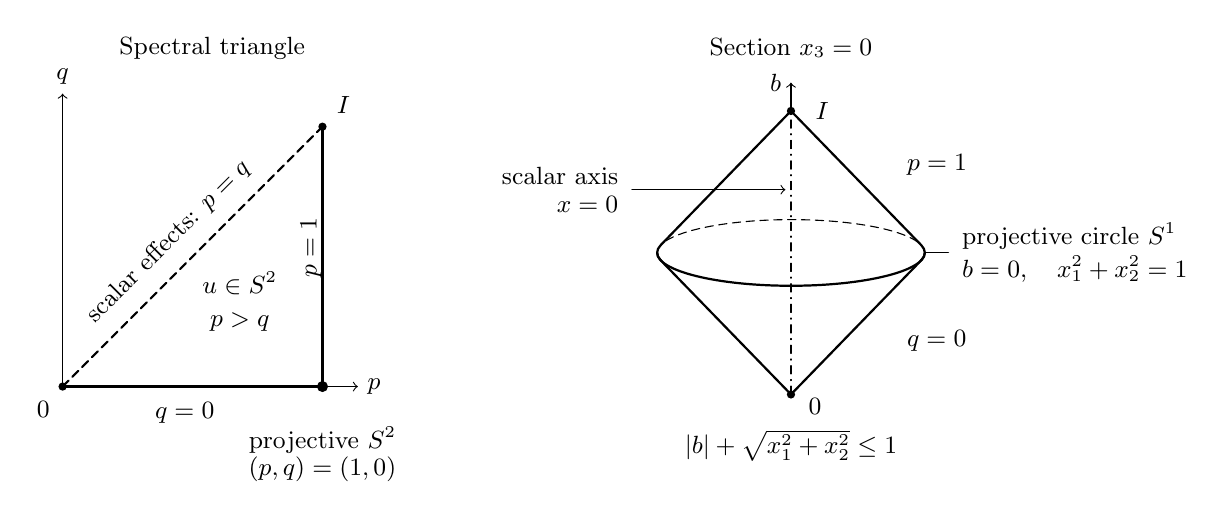
\begin{tikzpicture}[x=1cm,y=1cm,line cap=round,line join=round,
                    font=\small]
  % Left panel: exact ordered spectral triangle.
  \node at (1.9,4.30) {Spectral triangle};
  \draw[->,thin] (0,0) -- (3.75,0) node[right] {$p$};
  \draw[->,thin] (0,0) -- (0,3.72) node[above] {$q$};
  \draw[thick] (0,0) -- (3.3,0) -- (3.3,3.3);
  \draw[thick,densely dashed] (0,0) -- (3.3,3.3);
  \node[rotate=45,anchor=south] at (1.53,1.65)
    {scalar effects: $p=q$};
  \node[anchor=north] at (1.55,-0.08) {$q=0$};
  \node[rotate=90,anchor=south] at (3.41,1.77) {$p=1$};
  \node[align=center] at (2.25,1.08) {$u\in S^2$\\[1pt]$p>q$};
  \fill (0,0) circle (1.5pt);
  \fill (3.3,3.3) circle (1.5pt);
  \fill (3.3,0) circle (2pt);
  \node[anchor=north east] at (-0.04,-0.06) {$0$};
  \node[anchor=south west] at (3.36,3.34) {$I$};
  \node[anchor=north,align=center] at (3.30,-0.39)
    {projective $S^2$\\[-1pt]$(p,q)=(1,0)$};

  % Right panel: a three-dimensional section, shown in linear projection.
  % In local coordinates the map is
  % (x_1,x_2,b) -> (1.70*x_1,0.42*x_2+1.80*b).
  % The cone silhouette meets the projected unit circle at its exact
  % tangency points: sin(alpha)=0.42/1.80=7/30.
  \begin{scope}[shift={(9.25,1.70)}]
    \node at (0,2.60) {Section $x_3=0$};
    \pgfmathsetmacro{\tangentangle}{asin(7/30)}
    \pgfmathsetmacro{\tangentx}{1.70*cos(\tangentangle)}
    \pgfmathsetmacro{\tangenty}{0.42*sin(\tangentangle)}

    \draw[thin,densely dashed] (1.70,0)
      arc[start angle=0,end angle=180,x radius=1.70,y radius=0.42];
    \draw[thick] (-1.70,0)
      arc[start angle=180,end angle=360,x radius=1.70,y radius=0.42];
    \draw[thick] (-\tangentx,\tangenty) -- (0,1.80)
      -- (\tangentx,\tangenty);
    \draw[thick] (-\tangentx,-\tangenty) -- (0,-1.80)
      -- (\tangentx,-\tangenty);
    \draw[thick] (\tangentx,-\tangenty)
      arc[start angle=-\tangentangle,end angle=\tangentangle,
          x radius=1.70,y radius=0.42];
    \draw[thick] (-\tangentx,\tangenty)
      arc[start angle=180-\tangentangle,end angle=180+\tangentangle,
          x radius=1.70,y radius=0.42];

    \draw[thin,dash dot] (0,-1.80) -- (0,1.80);
    \draw[->,thin] (0,1.80) -- (0,2.16) node[left] {$b$};
    \fill (0,1.80) circle (1.5pt);
    \fill (0,-1.80) circle (1.5pt);
    \node[anchor=west] at (0.19,1.80) {$I$};
    \node[anchor=north west] at (0.10,-1.73) {$0$};
    \node[anchor=east,align=right] at (-2.07,0.80)
      {scalar axis\\[-1pt]$x=0$};
    \draw[->,thin] (-2.02,0.80) -- (-0.07,0.80);
    \node[anchor=west] at (1.35,1.12) {$p=1$};
    \node[anchor=west] at (1.35,-1.12) {$q=0$};
    \draw[thin] (1.71,0) -- (2.00,0);
    \node[anchor=west,align=left] at (2.05,0)
      {projective circle $S^1$\\[1pt]$b=0,\quad x_1^2+x_2^2=1$};
    \node[anchor=north] at (0,-2.13)
      {$|b|+\sqrt{x_1^2+x_2^2}\le1$};
  \end{scope}
\end{tikzpicture}
\caption{The four-dimensional effect body $|b|+|x|\le1$.
Each point of the spectral triangle with $p>q$ carries a direction
$u\in S^2$; on the scalar diagonal all directions represent the same
effect. The boundary pieces $q=0$ and $p=1$ meet at the projective stratum
$(p,q)=(1,0)$, which carries the full sphere $S^2$.
The right panel is a projection of the three-dimensional section
$x_3=0$; its equatorial circle is the intersection of that sphere
with the section.}
\label{fig:effectbody76}
\end{figure}

\section{The description entropy of all binary qubit effects}\label{sec:biasedentropy75}
Let
\[
 \mathfrak E=\{E=E^*\in\C^{2\times2}:0\le E\le I\}.
\]
An effect $E$ specifies the ordered measurement with effects $E,I-E$.
Write $\mathcal C_N(\mathfrak E,\delta)$ for its covering number under
$d_N$, allowing arbitrary legal memoryless centres of this interface,
and write $\mathcal C_N^{\mathrm{rat}}(\mathfrak E,\delta)$ when the
centres have rational Cartesian coordinates. Both eigenvalues and the
eigenspaces are charged. The spectral representation
$E=pP_u+q(I-P_u)$, $p\ge q$, represents a scalar effect only once,
independently of $u$.

\begin{theorem}[The full effect body]\label{thm:biasedcover75}
There are absolute constants $c,C,\delta_0>0$ such that, for every integer
$N\ge1$ and $0<\delta\le\delta_0$,
\begin{equation}\label{eq:biasedcover75}
 cN^2\log(N+2)\,\delta^{-4}
 \le \mathcal C_N(\mathfrak E,\delta)
 \le \mathcal C_N^{\mathrm{rat}}(\mathfrak E,\delta)
 \le CN^2\log(N+2)\,\delta^{-4}.
\end{equation}
Consequently the optimum fixed-length reusable payload is
\begin{equation}\label{eq:biasedbits75}
 2\log_2N+\log_2\log(N+2)+4\log_2(1/\delta)+O(1).
\end{equation}
The constants are uniform over the whole closed effect body, including
scalar, deterministic and projective effects. For rational accuracy
input, rational target data admit an exact rational encoder attaining
this order.
\end{theorem}
The logarithm records accumulation near the projective stratum, where
both outcome probabilities can approach their support endpoints.
We prove the upper bound by a finite rational construction and the
lower bound by separated families of projective-corner boxes.

\subsection{A rational spectral and angular code}
For $N\ge1$ and rational $0<\delta\le1/4$, put
\begin{equation}\label{eq:biasedspectralgrid75}
 B=\left\lceil\sqrt{64N/\delta^2}\right\rceil,\qquad
 s_i=\begin{cases}
 \displaystyle\frac{i^2}{B^2+i^2},&0\le i\le B,\\[2mm]
 \displaystyle1-\frac{(2B-i)^2}{B^2+(2B-i)^2},&B<i\le2B.
 \end{cases}
\end{equation}
Thus $0=s_0<s_1<\cdots<s_{2B}=1$. For $0\le j<i\le2B$ define
\begin{equation}\label{eq:biasedangulargrid75}
 K_{ij}^2=
 \frac{N(s_i-s_j)^2}
 {s_i(1-s_i)+s_j(1-s_j)+N^{-1}},\qquad
 A_{ij}=\max\left\{1,
      \left\lceil\sqrt{256K_{ij}^2/\delta^2}\right\rceil\right\}.
\end{equation}
Use the six signed stereographic charts
\begin{equation}\label{eq:biasedsphere75}
 u_a=\epsilon\frac{1-|z|^2}{1+|z|^2},\qquad
 u_b=\frac{2z_b}{1+|z|^2}\quad(b\ne a),\qquad
 a\in\{1,2,3\},\quad \epsilon\in\{-1,1\},
\end{equation}
with $z\in\{-A_{ij},\ldots,A_{ij}\}^2/A_{ij}$ for the spectral
pair $(s_i,s_j)$. Every chart word decodes to
$s_iP_u+s_j(I-P_u)$. A diagonal pair $i=j$ has the single word
$s_iI$. The exact number of words, including redundant chart words,
is
\begin{equation}\label{eq:biasedcapacity75}
 L_{N,\delta}=(2B+1)+
       \sum_{0\le j<i\le2B}6(2A_{ij}+1)^2.
\end{equation}

\begin{theorem}[Exact rational realization]\label{thm:biasedcodec75}
The words in \eqref{eq:biasedcapacity75} form a radius-$\delta/2$
cover of $\mathfrak E$ by legal rational effects, and
\begin{equation}\label{eq:biasedcapacitybound75}
 L_{N,\delta}\le C N^2\log(N+2)\,\delta^{-4}
\end{equation}
for an absolute $C$. If
\[
 E=\tfrac12\bigl((1+b)I+x\cdot\sigma\bigr),\qquad
 b\in\Q,\quad x\in\Q^3,\quad |b|+|x|\le1,
\]
then a covering word is computable by rational arithmetic and integer
comparisons. Its payload is one fixed-length index in the set of
\eqref{eq:biasedcapacity75}.
\end{theorem}
\begin{proof}
Write $f(t)=t^2/(1+t^2)$, $0\le t\le1$. For a probability in
$[0,1/2]$, round its inverse coordinate $t$ to the nearest multiple
of $1/B$; for a probability in $[1/2,1]$, use the reflected chart
$1-f(t)$. Choose the multiple of smaller magnitude at ties. This
defines a nondecreasing quantizer on $[0,1]$, so separately quantizing
$p\ge q$ preserves their order.

The square-root vector associated with $f(t)$ is
$(t,1)/\sqrt{1+t^2}$; its derivative has norm $1/(1+t^2)\le1$.
The reflected chart has the same bound. Hence the Euclidean
square-root distance between each probability and its quantization
is at most $1/(2B)$. If $H$ is this distance, the product-fidelity
inequality gives unhalved distance at most $2\sqrt N H$ between the
corresponding $N$-fold Bernoulli laws. The common two-coin programme
in Lemma~\ref{lem:spectralprojection75} therefore gives a spectral error
at most
\[
                         2\sqrt N/B\le\delta/4.
\]
This argument includes adaptive testers and entangled references.

If the quantized eigenvalues coincide, this completes the encoding.
Otherwise choose a signed chart whose distinguished coordinate has
maximal absolute value in the target direction. Its inverse coordinate
belongs to $[-1,1]^2$. Rounding its two coordinates to the grid of
denominator $A_{ij}$ gives angular error at most $2\sqrt2/A_{ij}$,
since geodesic distance is bounded by the length of the mapped
straight segment and the differential of stereographic projection has
norm at most two. The angular upper bound in Theorem~\ref{thm:biasedangular75}
gives error at most
\[
 \sqrt2 K_{ij}\frac{2\sqrt2}{A_{ij}}
                   \le\delta/4.
\]
The triangle inequality proves the covering assertion. Formula
\eqref{eq:biasedsphere75} preserves the unit sphere exactly, so every
decoded effect is legal and rational.

We verify exact computability even when the input eigenvalues are
irrational. Put $Q=|x|^2\in\Q$. The eigenvalues are
$(1+b\pm\sqrt Q)/2$. Each decision in the spectral rounding compares
one of these numbers with a rational threshold $f((k+1/2)/B)$ or its
reflection. Such a comparison is the sign of a rational number plus
or minus $\sqrt Q$; checking signs before squaring makes it an exact
rational comparison. If $Q=0$, the two quantized eigenvalues coincide.
Otherwise choose the smallest index $a$ maximizing $|x_a|$ and put
$\epsilon=\operatorname{sgn}(x_a)$. The inverse chart is
\[
                    z_b=\frac{x_b}{\sqrt Q+|x_a|}\quad(b\ne a).
\]
Its comparison with any rational rounding threshold again reduces
to the sign of a rational number plus a rational multiple of
$\sqrt Q$. The integers $B,A_{ij}$ are computed by integer squaring
and rational comparison. Thus no irrational normalization is required.
The decoder uses only the displayed rational formulae.

It remains to count the words. Set $m_i=\min(i,2B-i)$ and
$U=B^2/N$. Directly from \eqref{eq:biasedspectralgrid75},
\[
 \frac{m_i^2}{4B^2}\le s_i(1-s_i)\le\frac{m_i^2}{B^2},\qquad
 K_{ij}^2\le
          \frac{4NB^2}{m_i^2+m_j^2+U}.
\]
Each value of $m_i$ occurs at most twice. Since
$(2A_{ij}+1)^2\le C(1+K_{ij}^2/\delta^2)$, we obtain
\begin{equation}\label{eq:biasedlattice75}
 L_{N,\delta}\le CB^2+
 \frac{CNB^2}{\delta^2}
       \sum_{a,b=0}^{B}\frac1{a^2+b^2+U}.
\end{equation}
Here $U\ge1$. The part with $\max(a,b)\le\sqrt U$ is bounded by an
absolute constant. Each successive dyadic square ring contributes
at most another absolute constant. There are at most
$C\log(N+2)$ such rings, because $B/\sqrt U=\sqrt N$. Consequently
\[
              \sum_{a,b=0}^{B}\frac1{a^2+b^2+U}
                       \le C\log(N+2).
\]
Finally $B^2\le CN/\delta^2$, so \eqref{eq:biasedlattice75} proves
\eqref{eq:biasedcapacitybound75}. The support cutoff in the denominator
is retained throughout the count, including the endpoint grid words.
\end{proof}

\subsection{Packing the projective corner}
\begin{proof}[Proof of Theorem~\ref{thm:biasedcover75}]
The upper bound follows from Theorem~\ref{thm:biasedcodec75}. For a
real $\delta$, choose a rational $\delta'$ with
$\delta\le\delta'\le2\delta$ and use its radius-$\delta'/2$ code;
decrease $\delta_0$ to at most $1/8$. For the lower bound first let
$N\ge16$. For every
\[
                     t=8^j/N\le1/16,\qquad j\ge0,
\]
consider the effects with
\begin{equation}\label{eq:biasedcorner75}
 p=1-\alpha,\quad q=\beta,\quad
 t\le\alpha,\beta\le2t,\qquad
 u=u(z),\quad z\in[-1/4,1/4]^2,
\end{equation}
where $u(z)$ is the chart in \eqref{eq:biasedsphere75} with
$a=3,\epsilon=1$. On this square, spherical distance is bounded
above and below by absolute positive multiples of Euclidean distance
in $z$. Throughout \eqref{eq:biasedcorner75}, the eigenvalue gap is
at least $3/4$ and
\[
 p(1-p)\asymp q(1-q)\asymp t,\qquad
 p(1-p)+q(1-q)+N^{-1}\asymp t.
\]
The finite-distance comparison of Theorem~\ref{thm:biasedmetric75}
therefore supplies an absolute $c_1>0$ such that any two points in
this box satisfy
\begin{equation}\label{eq:biasedboxmetric75}
 d_N\ge c_1\min\left\{1,
       \sqrt{N/t}\,
       \bigl| (\alpha,\beta,z)-
              (\alpha',\beta',z')\bigr|_\infty\right\}.
\end{equation}
Choose an absolute sufficiently large $A$ and then an absolute
sufficiently small $\delta_0$. In each of the four coordinates take
a grid of spacing $A\delta\sqrt{t/N}$. Since $Nt\ge1$, this spacing
is at most half the width of either spectral interval when
$\delta\le\delta_0$. The resulting points have pairwise distance
at least $4\delta$ by \eqref{eq:biasedboxmetric75}, and their number
is at least
\[
 c\left(\frac{t}{\delta\sqrt{t/N}}\right)^2
   \left(\frac1{\delta\sqrt{t/N}}\right)^2
                         =cN^2\delta^{-4}.
\]

Points from different boxes are also uniformly separated. Indeed,
if $t'\ge8t$, then $\alpha'\ge t'$ and $\alpha\le2t\le t'/4$.
The spectral modulus of the corresponding upper eigenvalues is
bounded below by an absolute positive multiple of
$\sqrt{Nt'}\ge1$. The spectral noncancellation bound in
Theorem~\ref{thm:biasedmetric75} gives $d_N\ge c_2>0$.
Shrinking $\delta_0$ ensures that this is at least $4\delta$.
There are at least $c\log(N+2)$ permitted boxes. Their union is
therefore a $4\delta$-packing of cardinality
$cN^2\log(N+2)\delta^{-4}$.

For $1\le N<16$, use instead a fixed spectral rectangle
$5/8\le p\le3/4$, $1/4\le q\le3/8$ and the same angular chart.
Theorem~\ref{thm:biasedmetric75} gives a uniform local Euclidean lower
bound, and a grid of spacing $C\delta$ has at least $c\delta^{-4}$
points. The factor $N^2\log(N+2)$ is bounded on this finite range.
This proves the same lower estimate for all $N\ge1$.

A radius-$\delta$ ball about any legal centre contains at most one
point of a $4\delta$-packing, by the triangle inequality. Hence the
packing proves the lower bound with the stated centre convention.
Taking binary logarithms and rounding the index length proves
\eqref{eq:biasedbits75}.
\end{proof}

\subsection{The source of the logarithm}
The spectral and angular weights also give the following integral
form of the same accumulation. Put $v_p=p(1-p)$, $v_q=q(1-q)$ and
$\tau=N^{-1}$. Then
\begin{equation}\label{eq:biasedvolume75}
 \int_{0\le q\le p\le1}
 \frac{N^2(p-q)^2\,dp\,dq}
 {(v_p+v_q+\tau)\sqrt{(v_p+\tau)(v_q+\tau)}}
                         \asymp N^2\log(N+2).
\end{equation}
To verify this, near $p=1,q=0$ put $\alpha=1-p$, $\beta=q$.
After removing the factor $N^2$, the integrand is comparable to
\[
 \frac1{(\alpha+\beta+\tau)
             \sqrt{(\alpha+\tau)(\beta+\tau)}}.
\]
For $s=\alpha+\beta$, integration over $0\le\alpha\le s$ is
bounded above by an absolute constant times $1/(s+\tau)$.
For $s\ge2\tau$, restriction to $s/4\le\alpha\le3s/4$ gives the
matching lower bound. Integration in $s$ proves logarithmic growth.
Near the scalar endpoint $p=q=0$, the factor $(p-q)^2$ is at most
$(p+q)^2$, while $v_p+v_q\asymp p+q$; the remaining integral is
uniformly bounded. Complementation gives the same conclusion near
$p=q=1$. Away from these endpoint neighbourhoods,
$v_p+v_q$ is bounded below and the factors $v_p^{-1/2},v_q^{-1/2}$
are integrable. Bounded $N$ is absorbed into the constants.
Thus the extra logarithm is contributed by the projective corner.
The finite covering construction and packing above also include the
collapsed scalar coordinates, where the spectral representation
ceases to be a chart.

\section{Measurement discrimination, geometry, and learning}
\label{sec:matrixcomparison76}
The present binary interface retains the ordered classical outcome
and an arbitrary external reference, but no postmeasurement quantum
system from the device. This fixes the comparison with the
measurement-discrimination literature. The projective theorem of
Pucha\l a and collaborators \cite[Corollary~1 and Theorem~2]{PPKKO72}
gives an exact multiple-use formula with ancillary access. It is
used in the retained observable-readout theorem. The restricted
ancillary interface in Fiur\'a\v sek--Mi\v cuda \cite{FM75} leads
to a different comparison of adaptive and parallel probes.

Krawiec--Pawela--Pucha\l a \cite[Section~4]{KPP76} construct a pair
of nine-outcome qutrit rank-one POVMs that admit perfect adaptive
discrimination with two calls and no perfect discrimination by
any finite parallel experiment. Datta--Biswas--Saha--Augusiak
\cite[Theorems~3--5]{DBSA76} study entanglement-assisted
single-use discrimination, including perfect constructions and a
qubit entanglement advantage. Their qubit construction has three
outcomes. These are direct antecedents for general POVM
discrimination with a retained reference. They do not supply a
full binary-effect family covering law. Our comparison
\eqref{eq:matrixadaptivity76} permits an adaptive advantage and
controls its size uniformly in $N$ for fixed input dimension.

The differential argument in Lemma~\ref{lem:matrixpath76} belongs
to the established horizontal-gauge and channel-extension method
\cite{FI76,DKG67,DM76,KGAD76}. Yuan--Fung give the parallel path estimate
\cite[Section~III, equation~(26), PDF version~3]{YF76};
Sieniawski--Demkowicz-Dobrza\'nski integrate adaptive bounds
\cite[Section~IV.A]{SD76}. The binary Sylvester choice here gives the
specific regularized variance $M(I-M)$, which can be integrated
explicitly and matched by compressed nonadaptive tests. The
inverse-Sylvester expressions of Bures geometry
\cite{Dittmann76} and its spectral integration
\cite{SZGeom76} are related methods. Our form acts on the effect
displacement $H$ with variance $V=M(I-M)$; it is not the ordinary
Bures pullback under $M\mapsto V$, whose differential would be
$H-MH-HM$. The operational-ball lemma and the nested endpoint
integral are both required for Theorem~\ref{thm:matrixcover76}.

Mele--Bittel \cite[Theorem~I.1]{MB67} prove the
fixed-confidence channel-learning bound
$O(d_{\rm in}d_{\rm out}k\epsilon^{-2})$ for Kraus rank at
most $k$ and $0<\epsilon<1$. Their binary specialization
\cite[Lemmas~III.7--III.8 and Corollary~III.9]{MB67} gives
\[
 \|\mathcal M_E-\mathcal M_F\|_\diamond
     =2\|E-F\|_{\rm op},\qquad
 M=1024d^2\epsilon^{-2}
       +O(d\epsilon^{-2}\log(1/\eta)),
\]
with $\|\widehat E-E\|_{\rm op}\le\epsilon$ and probability
at least $1-\eta$, provided $\eta>4e^{-4d^2}$.
The channel-rank bound is $k=2d$; no effect-rank assumption
is imposed. Their channel calls prepare independent maximally
entangled probes in parallel, followed by collective processing
of the resulting Choi states. The learner has no measurement-
environment access. For arbitrary confidence,
\cite[Remark~III.4]{MB67} gives the repetition bound
$O(d^2\epsilon^{-2}\log(1/\eta))$.
The dimension lower bound matches at fixed accuracy; it is
distinct from their separate accuracy lower bound.

Zambrano--Ramos-Calderer--Kueng \cite[Definition~1]{ZRK76}
use the worst-input one-use outcome total variation, denoted
$d_{\rm op}$. Their Theorem~2, equation~(13), gives
\[
 M\ge
 \frac{8(d^2+\epsilon(d^2+1)/6)}{\epsilon^2}
 \log\frac{2^{L+1}9^{2d}}{\eta}
\]
as a sufficient sample size for error $\epsilon$ and
confidence $1-\eta$, using known probes from a global
$2$-design and classical least-squares reconstruction followed
by projection onto the POVM body. Calls are nonadaptive and
single-copy, without retained references or entanglement
between calls. The result holds for arbitrary effect ranks
and $L$ outcomes. Their Theorem~9 gives the corresponding
$\Omega((d^3+d^2L)\epsilon^{-2})$ lower bound at constant
confidence within that access model. For $L=2$,
$d_{\rm op}(E,F)=\|E-F\|_{\rm op}$.

Thus both works already provide a common estimator of an
unknown binary measurement. To compare their stated guarantees
with the present loss, the hybrid inequality gives
\[
 d_N(\mathcal M_E,\mathcal M_{\widehat E})
      \le 2N\|E-\widehat E\|_{\rm op}.
\]
Substituting $\epsilon=\delta/(2N)$ into either cited
binary guarantee gives a sufficient training budget
$O_d(N^2\delta^{-2}\log(1/\eta))$.
This substitution certifies a sufficient budget; it makes no converse
assertion about those estimators under the future-use loss.
Theorem~\ref{thm:matrixlearning77} proves
$\Theta_d(N\delta^{-2}\log(1/\eta))$ directly for $d_N$,
uniformly over the complete binary matrix effect body for each fixed
$d$, for
$N\ge1$, $0<\delta\le\delta_0$, and $0<\eta\le1/8$.
Its training procedure chooses entangled input blocks of length
at most $N$ using the observed record, and returns one legal
classical estimate. The lower bound allows arbitrary retained
references, adaptive controls, and bounded public stopping.
The explicit upper bound is $Cd^4N\delta^{-2}\log(d/\eta)$;
its dimension dependence is not asserted to be sharp. Calibration of
both support endpoints and noise-adapted compression learning are
what permit the statistical theorem to share the full matrix scope
of the metric theorem.
Multiscale phase estimation and robust phase recovery are
established techniques \cite{HB76,KLY76}. Our proof supplies its
own small-cone argument and conditional confidence allocation;
it does not invoke the numerical unwrapping threshold corrected
by the erratum to \cite{KLY76}. Randomized signs remove the
unknown bias exactly, and empirical amplitudes choose the
entangled block length without a supplied noise parameter.
The qubit subprocedure is common to all unknown qubit effects.
The calibrated compression construction extends common learning to
the full matrix body in every fixed dimension. The pair-dependent tests used in the matrix
metric comparison and the supplied-target exact encoder retain
their separate roles.

The deterministic rational construction in
Theorem~\ref{thm:matrixcodec77} adds a finite exact selection rule
to the optimal-order covering theorem. Its exhaustive computation is
accounted for separately from the payload; no efficient high-dimensional
encoder or optimal arithmetic complexity is inferred.

All matrix entropy constants are for fixed dimension and small
error. The proof includes every rank and spectral multiplicity
of the binary effect body. Multi-outcome POVMs, residual quantum
outputs, sharp growing-dimension minimax and entropy laws, and full submaximal-error
matrix coverings require additional arguments. The inherited
full-error preparation and fixed-readout results retain their
own stated ranges.

\appendix
% Verbatim self-contained prerequisite excerpt from sections/49-noisy-readout-crossover.tex.
% The complete section, including conditional-output results, remains in main.tex.
\section{A noise-uniform readout transition}\label{sec:noisyreadout73}
The dependence on the readout basis can change scale when noise approaches
an extremal measurement. We determine that transition in a fixed
one-dimensional family, without a positive spectral margin uniform in
the noise. The proof is a finite-distance argument; no conclusion is
inferred merely from a Fisher-information calculation.

Let $\sigma_1,\sigma_2$ be the first two Pauli matrices. For
$\theta\in\R/(2\pi\Z)$ and a public visibility $0\le\lambda\le1$, put
\begin{equation}\label{eq:noisyfamily73}
 E_{\theta,\lambda}^{\pm}
 =\frac12\bigl(I\pm\lambda(\cos\theta\,\sigma_1+
                                  \sin\theta\,\sigma_2)\bigr),\qquad
 \mathcal M_{\theta,\lambda}^{\pm}(X)=\tr(E_{\theta,\lambda}^{\pm}X).
\end{equation}
Both outcome labels are retained. The output quantum system is
one-dimensional. In particular, $\theta$ and $\theta+\pi$ are not
identified by an outcome relabelling. Let $h(\theta,\phi)\in[0,\pi]$
be circular distance and set
\begin{equation}\label{eq:noisyscale73}
 \eta=1-\lambda^2,\qquad
 K_{N,\lambda}=\lambda\sqrt{N\min\{N,\eta^{-1}\}},\qquad N\ge1,
\end{equation}
where $\eta^{-1}=+\infty$ at $\lambda=1$. Thus $K_{N,1}=N$ and
$K_{N,0}=0$. The visibility may depend arbitrarily on $N$ and the
requested error; it is not a target coordinate charged in this theorem.

Write $\mathcal C_{N,\lambda}(\delta)$ for the least number of legal
memoryless binary instruments of this interface whose $d_N$-balls of
radius $\delta$ cover all targets in \eqref{eq:noisyfamily73}.
Centres need not belong to the displayed family. Define
$\mathcal C^{\mathrm{rat}}_{N,\lambda}(\delta)$ by restricting centres
to family members with rational $\cos\theta,\sin\theta$; rational
visibility then gives rational effects. A constant in the following
statement is independent of all three parameters $N,\lambda,\delta$.

\begin{theorem}[Noise-uniform finite-use coding]\label{thm:noisycoding73}
For all $N\ge1$, $0\le\lambda\le1$, and all pairs of angles,
\begin{equation}\label{eq:noisymetric73}
 \frac1{64}\min\{1,K_{N,\lambda}h(\theta,\phi)\}
 \le d_N(\mathcal M_{\theta,\lambda},\mathcal M_{\phi,\lambda})
 \le\min\{2,K_{N,\lambda}h(\theta,\phi)\}.
\end{equation}
There are absolute $c,C>0$ such that, for $0<\delta\le2^{-10}$,
\begin{equation}\label{eq:noisycover73}
 c\left(1+\frac{K_{N,\lambda}}\delta\right)
 \le\mathcal C_{N,\lambda}(\delta)
 \le\mathcal C^{\mathrm{rat}}_{N,\lambda}(\delta)
 \le C\left(1+\frac{K_{N,\lambda}}\delta\right).
\end{equation}
Consequently the optimum fixed-length reusable payload is
\begin{equation}\label{eq:noisybits73}
 \log_2\left(1+\frac{K_{N,\lambda}}\delta\right)+O(1).
\end{equation}
The upper construction is an exact rational algorithm on rational
visibility, tolerance and unit-circle input coordinates. At $\lambda=0$
the family is a singleton and its optimum payload is zero.
\end{theorem}
The constants and the additive remainder are uniform up to the erased
and projective endpoints. In contrast, they do not assert an optimal
leading constant, a large-error coherent covering law, or a coding law
in which an unknown visibility is also encoded.

\subsection{A two-point programme with its noise dependence retained}
\begin{lemma}[An adaptive upper modulus]\label{lem:noisyupper73}
Let $h=h(\theta,\phi)$ and $a=\lambda\sin(h/2)$. If $\eta>0$, then
\begin{equation}\label{eq:noisyfiniteupper73}
 d_N(\mathcal M_{\theta,\lambda},\mathcal M_{\phi,\lambda})
 \le\min\left\{2,\ 2Na,\
             2\sqrt{1-\left(\frac{\eta}{\eta+a^2}\right)^N}\right\}.
\end{equation}
For $\eta=0$ the bound $\min\{2,2Na\}$ remains valid.
\end{lemma}
\begin{proof}
The difference of the two positive-outcome effects has operator norm
$a$. On a bipartite input state, the two output blocks of the difference
are $B$ and $-B$, where
$B=\tr_A[((E^+_{\theta,\lambda}-E^+_{\phi,\lambda})\otimes I)\rho]$.
Duality against Hermitian contractions gives $\|B\|_1\le a$.
An eigenstate of the effect difference attains equality. Hence
$d_1=2a$, including reference assistance. Replacing the calls one at a
time and using trace-norm contraction proves $d_N\le2Na$ for every
common adaptive tester.

Choose angle representatives with difference $h$ and let $u,v$ be the
unit vectors along their midpoint and its oriented perpendicular in
the equatorial plane. The two Bloch vectors are $m\pm av$, where
$m=\lambda\cos(h/2)u$. Put
$b=(1-\|m\|^2)^{1/2}=(\eta+a^2)^{1/2}$.
The two Bloch vectors $m\pm bv$ have norm one, so they define two legal
binary projective instruments, say $\mathcal A_+$ and $\mathcal A_-$.
The target pair is exactly the two mixtures of these same instruments
with programme laws
\[
 p_\pm=\bigl((1\pm t)/2,(1\mp t)/2\bigr),\qquad t=a/b.
\]
This construction depends on the pair, which is permissible in a
metric upper bound. It is not one fixed processor for the whole circle.

For a fixed tester, first supply $N$ independent programme bits and,
at each requested call, apply the indicated $\mathcal A_+$ or
$\mathcal A_-$. All subsequent operations, including the reference,
feedback and a stopping rule, are a common channel of these bits.
Unused bits are discarded. The root fidelity of $p_+,p_-$ is
$\sqrt{1-t^2}$. Purifying the classical laws and using contraction gives
\[
 \|p_+^{\otimes N}-p_-^{\otimes N}\|_1
 \le2\sqrt{1-(1-t^2)^N}.
\]
This also follows directly from the classical fidelity inequality.
Substitution proves \eqref{eq:noisyfiniteupper73}.
Finally $1-(1-t^2)^N\le Nt^2$ and $a\le\lambda h/2$ imply
\[
 d_N\le\min\{N\lambda h,\sqrt{N/\eta}\,\lambda h,2\}.
\]
The limiting projective bound is supplied by the hybrid estimate,
not by division by zero.
\end{proof}
Classical simulation by common extremal channels and the effect of
noise on the Heisenberg scale are established methods
\cite{DKG67}. Environment/programme-state processing under adaptive
use is also an established framework \cite{DW72,WBHK72,WW72}.
The point needed here is the exact two-point expression
\eqref{eq:noisyfiniteupper73} and its uniform conversion to a family
cover, rather than a new claim about the origin of those methods.

\subsection{Finite entangled blocks and a binary product estimate}
\begin{lemma}[Symmetric Bernoulli products]\label{lem:bernoullimajority73}
Let $P_\pm$ be Bernoulli laws with success probabilities
$(1\pm a)/2$, where $0\le a\le1$. For every integer $m\ge1$,
\begin{equation}\label{eq:bernoullimajority73}
 \|P_+^{\otimes m}-P_-^{\otimes m}\|_1
                   \ge\tfrac12\min\{1,a\sqrt m\}.
\end{equation}
\end{lemma}
\begin{proof}
Retain the largest odd number $r=2j+1\le m$ of coordinates, so
$r\ge m/2$. For their majority event write
$g_r(a)=P_+(\text{majority})-P_-(\text{majority})$.
Differentiating the finite binomial sum and cancelling consecutive
terms gives
\[
 g_r'(a)=r\binom{2j}{j}4^{-j}(1-a^2)^j.
\]
For $j\ge1$, the bound $\binom{2j}{j}4^{-j}\ge1/(2\sqrt j)$
follows by induction: the ratio of consecutive left sides is
$(2j+1)/(2j+2)\ge\sqrt{j/(j+1)}$. For
$0\le a\le r^{-1/2}$, Bernoulli's inequality gives
$(1-a^2)^j\ge1-j/r\ge1/2$. Thus
$g_r'(a)\ge\sqrt r/(2\sqrt2)$ on that interval. The case $r=1$
is immediate. Integration from zero and monotonicity yield
$g_r(a)\ge(2\sqrt2)^{-1}\min\{1,a\sqrt r\}$.
Unhalved distance is at least twice this event difference; using
$r\ge m/2$ proves the stated bound.
\end{proof}

\begin{lemma}[A noise-uniform pairwise witness]\label{lem:noisylower73}
The lower inequality in \eqref{eq:noisymetric73} is witnessed by
nonadaptive entangled blocks, each of at most $N$ qubits, followed by
classical parity and majority processing.
\end{lemma}
\begin{proof}
A block of $k$ inputs is prepared in
$(|0\rangle^{\otimes k}+e^{i\alpha}|1\rangle^{\otimes k})/\sqrt2$.
Multiplying the $k$ output signs of \eqref{eq:noisyfamily73} has mean
$\lambda^k\cos(k\theta-\alpha)$. This identity follows by applying
$\bigotimes_{i=1}^k(E^+-E^-)$ to the two off-diagonal terms of the
block density matrix. For the two hypotheses choose the one common
phase $\alpha=k(\theta+\phi)/2+\pi/2$. Their parity laws then have
opposite biases of magnitude
\begin{equation}\label{eq:ghzbias73}
                        a_k=\lambda^k|\sin(kh/2)|.
\end{equation}
Repeating $m=\lfloor N/k\rfloor$ independent blocks and ignoring
remaining calls is an admissible tester. Its unhalved output distance
is at least $\tfrac12\min\{1,\sqrt m\,a_k\}$ by
Lemma~\ref{lem:bernoullimajority73}. The phase and block size may depend
on the pair, but never on the unknown hypothesis or a private outcome.

Assume $\lambda>0$ and put
$T=\min\{N,\eta^{-1}\}$, $k_0=\lfloor T\rfloor$. Then
$T/2\le k_0\le T$. For every $1\le k\le k_0$,
\begin{equation}\label{eq:visibilityblock73}
                              \lambda^k\ge\lambda/2.
\end{equation}
Indeed, when $0<\eta<1$, the inequality
$\log(1-\eta)\ge-\eta/(1-\eta)$ and
$k-1\le\eta^{-1}-1$ give $(k-1)\log\lambda\ge-1/2$.
At $\eta=0$ the assertion is immediate.

If $h\le1/k_0$, choose $k=k_0$. Since
$\sin(kh/2)\ge kh/\pi$ and $m\ge N/(2k)$, we obtain
\[
 \sqrt m\,a_k\ge
 \frac{\lambda\sqrt{Nk_0}}{2\pi\sqrt2}h
 \ge\frac{K_{N,\lambda}}{4\pi}h.
\]
This gives a lower constant $1/(8\pi)$.
If $k_0=1$, use $k=1$ for all $h\le\pi$ instead. Now $T<2$
unless $T=1$, and $\sqrt N\lambda\sin(h/2)\ge
K_{N,\lambda}h/(\pi\sqrt2)$; this is stronger than required.

It remains that $k_0\ge2$ and $h>1/k_0$. Here
$\lambda\ge1/\sqrt2$. Choose $k=\max\{1,\lfloor1/h\rfloor\}$.
Then $k\le k_0$ and $1/2\le kh\le\pi$. Equations
\eqref{eq:ghzbias73} and \eqref{eq:visibilityblock73} give
$a_k\ge1/(4\pi\sqrt2)$. Even one such block has distance at least
$1/(8\pi\sqrt2)>1/64$. The three cases prove the claim.
For $\lambda=0$ both sides of the desired inequality vanish.
\end{proof}

\subsection{Covering and exact rational realization}
\begin{proof}[Proof of Theorem~\ref{thm:noisycoding73}]
The metric assertion follows from the preceding lemmas. For a lower
cover choose points on the circle with circular separation at least
$256\delta/K_{N,\lambda}$ whenever that quantity is at most $\pi$.
An equally spaced packing has at least a fixed constant times
$K_{N,\lambda}/\delta$ points. Every two points have $d_N$-distance
at least $4\delta$, because $256\delta\le1/4$.
No radius-$\delta$ ball, even about an arbitrary legal instrument, can
contain two such points. If the required angular separation exceeds
$\pi$, the trivial lower bound one suffices, with a smaller absolute
constant. This proves the first inequality in \eqref{eq:noisycover73}.

For the upper bound use the two rational semicircle charts
\begin{equation}\label{eq:circlechart73}
 z_s(t)=s\left(\frac{1-t^2}{1+t^2},\frac{2t}{1+t^2}\right),
                 \qquad s\in\{-1,1\},\quad -1\le t\le1.
\end{equation}
Each chart has angular speed $2/(1+t^2)\le2$. Round $t$ to the
nearest $j/B$, $-B\le j\le B$, with a fixed rule at ties. The
circular error is at most $1/B$. Thus any integer
$B\ge\max\{1,K_{N,\lambda}/\delta\}$ yields a cover with at most
$4B+2$ centres. For rational inputs, an entirely rational choice is
\begin{equation}\label{eq:noisygrid73}
 B=\max\left\{1,\min\left\{
   \left\lceil\frac{4N\lambda}{\delta}\right\rceil,
   \left\lceil\sqrt{\frac{16N\lambda^2}{\eta\delta^2}}\right\rceil
                                  \right\}\right\},
\end{equation}
omitting the second entry when $\eta=0$. Integer squaring and rational
comparison compute the ceiling square root exactly. Both entries are
ceilings of the corresponding real bounds, so their minimum is
$\lceil4K_{N,\lambda}/\delta\rceil$.
For $z=(x,y)$ on the rational unit circle choose $s=1$ when $x\ge0$
and $s=-1$ otherwise, and set $t=sy/(1+sx)$. Its denominator is at
least one, so it is rational and belongs to $[-1,1]$.

The chart digit $(s,j)$ determines a legal effect pair with eigenvalues
$(1\pm\lambda)/2$. No approximate positivity test, irrational
normalization or search over real angles is needed. A fixed-length
index over $4B+2$ slots includes the chart sign. Its length gives
\eqref{eq:noisybits73}. Redundant chart endpoints cause at most a
constant overhead. At $\lambda=0$ dispense with the chart and emit the
single fair, input-erasing measurement.
\end{proof}

\begin{corollary}[A continuous family of horizon exponents]\label{cor:noisyexponents73}
Fix $0<\delta\le2^{-10}$. If $\lambda_N\to1$ and
$1-\lambda_N^2=N^{-\alpha+o(1)}$ for $\alpha\ge0$, then
\[
 \frac{\log_2\mathcal C_{N,\lambda_N}(\delta)}{\log_2N}
                       \longrightarrow\frac{1+\min\{\alpha,1\}}2.
\]
If $\lambda_N=N^{-\beta+o(1)}\to0$, with $\beta\ge0$, the limit is
$\max\{1/2-\beta,0\}$. The projective and erased endpoints have
coefficients one and zero, respectively.
\end{corollary}
\begin{proof}
Substitute the two regimes in \eqref{eq:noisyscale73} and use
\eqref{eq:noisycover73}. The term $1+K/\delta$ handles a vanishing
or subpolynomial scale without taking the logarithm of zero.
\end{proof}

\begin{thebibliography}{99}
\bibitem{Watrous65} J. Watrous, \emph{The Theory of Quantum Information},
Cambridge University Press, 2018. Theorems~2.22 and~2.26
(Choi criteria), Corollary~3.40 (trace-norm contraction),
and Section~3.3, equation~(3.306) (hybrid comparison).
\bibitem{PLS66} T. Surawy-Stepney, J. Kahn, R. Kueng and M. Gu\c{t}\u{a},
Projected least-squares quantum process tomography,
\emph{Quantum} \textbf{6} (2022), 844;
arXiv:2107.01060v2, 18 October 2022.
\bibitem{Gutoski66} G. Gutoski,
On a measure of distance for quantum strategies,
\emph{J. Math. Phys.} \textbf{53} (2012), 032202;
arXiv:1008.4636v4, 14 March 2012.
\bibitem{NZGB67} S. G. Naik, M. Zartab, N. Gisin and M. Banik,
No-Go Theorem for Generic Simulation of Qubit Channels with Finite
Classical Resources, arXiv:2501.15807v2 (16 July 2025),
Theorems~2 and~5.
\bibitem{MB67} A. A. Mele and L. Bittel,
Optimal learning of quantum channels in diamond distance,
arXiv:2512.10214v3 (2026), Theorem~I.1, Lemmas~III.7--III.8,
Corollary~III.9 and Sections~III.1.1, IV.1.1.
\bibitem{OG67} A. Oufkir and F. Girardi,
Improved Lower Bounds for Learning Quantum Channels in Diamond
Distance, arXiv:2601.04180v4 (2026).
\bibitem{DKG67} R. Demkowicz-Dobrza\'nski, J. Ko\l ody\'nski
and M. Gu\c{t}\u{a}, The elusive Heisenberg limit in quantum-enhanced
metrology, \emph{Nature Communications} \textbf{3} (2012), 1063.
DOI: 10.1038/ncomms2067; arXiv:1201.3940v2, equations~(4)--(6)
(classical simulation), equations~(10)--(13) (channel extension),
and the classical-simulation argument in Methods.
\bibitem{YBCH68} Y.~Yang, G.~Bai, G.~Chiribella and M.~Hayashi,
Compression for quantum population coding,
\emph{IEEE Transactions on Information Theory} \textbf{64} (2018), no.~7,
doi:10.1109/TIT.2017.2788407;
arXiv:1701.03372v8.
\bibitem{SHW68} F.~Salek, M.~Hayashi and A.~Winter,
Usefulness of adaptive strategies in asymptotic quantum channel
 discrimination, \emph{Phys. Rev. A} \textbf{105} (2022), 022419;
arXiv:2011.06569v3 (17 March 2024).
\bibitem{CMW70} T.~Cooney, M.~Mosonyi and M.~M.~Wilde,
Strong converse exponents for a quantum channel discrimination problem
and quantum-feedback-assisted communication,
arXiv:1408.3373v3 (26 February 2016), p.~5 and Sections~4.1--4.2.
\bibitem{Acin70} A.~Ac\'in,
Statistical distinguishability between unitary operations,
\emph{Phys. Rev. Lett.} \textbf{87} (2001), 177901.
DOI: 10.1103/PhysRevLett.87.177901.
\bibitem{DFY70} R.~Duan, Y.~Feng and M.~Ying,
Entanglement is not necessary for perfect discrimination between
unitary operations, \emph{Phys. Rev. Lett.} \textbf{98} (2007), 100503.
DOI: 10.1103/PhysRevLett.98.100503.

\bibitem{DW72} S. Das and M. M. Wilde,
Quantum reading capacity: General definition and bounds,
\emph{IEEE Trans. Inform. Theory} \textbf{65} (2019), 7566--7583;
arXiv:1703.03706v3; doi:10.1109/TIT.2019.2929925.
\bibitem{WBHK72} M. M. Wilde, M. Berta, C. Hirche and E. Kaur,
Amortized channel divergence for asymptotic quantum channel discrimination,
\emph{Lett. Math. Phys.} \textbf{110} (2020), 2277--2336;
arXiv:1808.01498v2; doi:10.1007/s11005-020-01297-7.
\bibitem{WW72} X. Wang and M. M. Wilde,
Resource theory of asymmetric distinguishability for quantum channels,
\emph{Phys. Rev. Research} \textbf{1} (2019), 033169;
arXiv:1907.06306v2; doi:10.1103/PhysRevResearch.1.033169.
\bibitem{PPKKO72} Z. Pucha\l a, \L. Pawela, A. Krawiec, R. Kukulski and
M. Oszmaniec, Multiple-shot and unambiguous discrimination of von Neumann
measurements, \emph{Quantum} \textbf{5} (2021), 425;
arXiv:1810.05122v4; doi:10.22331/q-2021-04-06-425.


\bibitem{SZ74} M. Sedl\'ak and M. Ziman,
Optimal single-shot strategies for discrimination of quantum measurements,
\emph{Phys. Rev. A} \textbf{90} (2014), 052312;
arXiv:1408.0934; doi:10.1103/PhysRevA.90.052312.
Section VI, Example 4, equation (37).
\bibitem{PPKK74} Z. Pucha\l a, \L. Pawela, A. Krawiec and R. Kukulski,
Strategies for optimal single-shot discrimination of quantum measurements,
\emph{Phys. Rev. A} \textbf{98} (2018), 042103;
arXiv:1804.05856; doi:10.1103/PhysRevA.98.042103. Theorem 1.
\bibitem{FM75} J.~Fiur\'a\v sek and M.~Mi\v cuda,
Optimal two-copy discrimination of quantum measurements,
\emph{Phys. Rev. A} \textbf{80} (2009), 042312;
arXiv:0909.2940; doi:10.1103/PhysRevA.80.042312.

\bibitem{KPP76} A.~Krawiec, \L.~Pawela and Z.~Pucha\l a,
Discrimination of POVMs with rank-one effects,
\emph{Quantum Information Processing} \textbf{19} (2020), 428;
arXiv:2002.05452v1; doi:10.1007/s11128-020-02883-3.
\bibitem{DBSA76} C.~Datta, T.~Biswas, D.~Saha and R.~Augusiak,
Perfect discrimination of quantum measurements using entangled systems,
\emph{New Journal of Physics} \textbf{23} (2021), 043021;
arXiv:2012.07069v2; doi:10.1088/1367-2630/abecaf.
\bibitem{FI76} A.~Fujiwara and H.~Imai,
A fibre bundle over manifolds of quantum channels and its application
to quantum statistics,
\emph{J. Phys. A: Math. Theor.} \textbf{41} (2008), 255304;
doi:10.1088/1751-8113/41/25/255304. Theorems~4 and~5.
\bibitem{DM76} R.~Demkowicz-Dobrza\'nski and L.~Maccone,
Using entanglement against noise in quantum metrology,
\emph{Phys. Rev. Lett.} \textbf{113} (2014), 250801;
arXiv:1407.2934v3; doi:10.1103/PhysRevLett.113.250801.
\bibitem{KGAD76} S.~Kurdzia\l ek, W.~G\'orecki, F.~Albarelli
and R.~Demkowicz-Dobrza\'nski,
Using adaptiveness and causal superpositions against noise in quantum metrology,
\emph{Phys. Rev. Lett.} \textbf{131} (2023), 090801;
arXiv:2212.08106v2; doi:10.1103/PhysRevLett.131.090801.
\bibitem{YF76} H.~Yuan and C.-H.~F.~Fung,
Fidelity and Fisher information on quantum channels,
arXiv:1506.00819v3 (2017), Section~III, equation~(26).
\bibitem{SD76} S.~Sieniawski and R.~Demkowicz-Dobrza\'nski,
Adaptive quantum channel discrimination using methods of quantum metrology,
\emph{New Journal of Physics} \textbf{28} (2026), 024502;
arXiv:2510.15506v3; doi:10.1088/1367-2630/ae3edd.
\bibitem{Dittmann76} J.~Dittmann,
Explicit formulae for the Bures metric,
\emph{J. Phys. A: Math. Gen.} \textbf{32} (1999), 2663--2670;
doi:10.1088/0305-4470/32/14/007;
arXiv:quant-ph/9808044, entitled
\emph{Note on explicit formulae for the Bures metric}.
\bibitem{SZGeom76} H.-J.~Sommers and K.~\.{Z}yczkowski,
Bures volume of the set of mixed quantum states,
\emph{J. Phys. A: Math. Gen.} \textbf{36} (2003), 10083--10100;
arXiv:quant-ph/0304041v3; doi:10.1088/0305-4470/36/39/308.
\bibitem{ZRK76} L.~Zambrano, S.~Ramos-Calderer and R.~Kueng,
Fast quantum measurement tomography with optimal error bounds,
\emph{Quantum} \textbf{10} (2026), 2162;
arXiv:2507.04500v3; doi:10.22331/q-2026-07-15-2162.
\bibitem{BDPS76} A.~Bisio, G.~M.~D'Ariano, P.~Perinotti and M.~Sedl\'ak,
Quantum learning algorithms for quantum measurements,
\emph{Physics Letters A} \textbf{375} (2011), 3425--3434;
arXiv:1103.0480v2; doi:10.1016/j.physleta.2011.08.002.
\bibitem{HB76} B.~L.~Higgins, D.~W.~Berry, S.~D.~Bartlett,
M.~W.~Mitchell, H.~M.~Wiseman and G.~J.~Pryde,
Demonstrating Heisenberg-limited unambiguous phase estimation
without adaptive measurements,
\emph{New Journal of Physics} \textbf{11} (2009), 073023;
arXiv:0809.3308v4; doi:10.1088/1367-2630/11/7/073023.
\bibitem{KLY76} S.~Kimmel, G.~H.~Low and T.~J.~Yoder,
Robust calibration of a universal single-qubit gate set via robust phase estimation,
\emph{Phys. Rev. A} \textbf{92} (2015), 062315;
doi:10.1103/PhysRevA.92.062315;
erratum, \emph{Phys. Rev. A} \textbf{104} (2021), 069901,
doi:10.1103/PhysRevA.104.069901; arXiv:1502.02677v3.

\end{thebibliography}

\end{document}
